\chapter{Demonstration Cases and Benchmarking}\label{ch:demonstration}

Basic verification of the integrated behavior of the components in the \Cyder 
model was achieved with a suite of toy base cases and a suite of physics 
demonstrating validation comparisons. 

The toy base cases were simplistic simulations that were intended 
to verify the fundamental behavior of the mass balance models and mass transfer 
modes. These aphysical but informative simulations were run to asses the simplistic 
behavior of an assembly of \Cyder components within a simplistic \Cyclus 
simulation.

The physics demonstrations, on the other hand, sought to demonstrate that the 
dominant physics of repository performance were captured as intended by the 
various contaminant and thermal transport models implemented in \Cyder.

\section{Radionuclide Transport Base Cases}\label{sec:nuclide_base_cases}
\subsection{No Release Problem Specification}
The no release base cases tested basic null containment transport behavior of 
all the radionuclide transport models at each component interface. This test 
neglected thermal transport and capacity estimation to simplify validation. 

The problem design includes : 
\begin{itemize}
\item[A source facility providing one waste stream per timestep]
\item[A legislated repository capacity of 5 1kg waste streams]
\item[A waste form Component] 
\item[A waste package Component]
\item[A buffer Component]
\item[A far field Component]
\end{itemize}

\subsubsection{Degradation Rate Model}
The Degradation Rate model should not release contaminants if the degradation 
rate is 0. Thus, four simulations were run to demonstrate the containment 
behavior at the Waste Form, Waste Package, Buffer, and Far Field interfaces. 

\input{./chapters/demonstration/dr_no_release_tab}

\subsubsection{Mixed Cell Model}

\begin{table}
\centering
\begin{tabular}{|l|c|c|r|}
  \hline
  \multicolumn{4}{c}{\textbf{Mixed Cell Model No Release Contaminant Transport}}\\
  \hline
  \textbf{Case}  &  \textbf{Component} &  \textbf{Degradation Rate} & \textbf{Expected 10 yrs} & \textbf{Actual 10 yrs}\\
  \textbf{ID}    & \textbf{[Type]} &  \textbf{$[yr^{-1}]$}  &  $[\%]$  & $[\%]$\\
  \hline
  MCI     &  WF    &  0   & 1\\
          &  WP    &  0.1 & 0\\
          &  BUFF  &  0.1 & 0\\
          &  FF    &  0.1 & 0\\
  \hline
  MCII    &  WF    &  0.1 & 0\\
          &  WP    &  0   & 1\\
          &  BUFF  &  0.1 & 0\\
          &  FF    &  0.1 & 0\\
  \hline
  MCIII   &  WF    &  0.1 & 0\\
          &  WP    &  0.1 & 0\\
          &  BUFF  &  0   & 1\\
          &  FF    &  0.1 & 0\\
  \hline
  MCIV    &  WF    &  0.1 & 0\\
          &  WP    &  0.1 & 0\\
          &  BUFF  &  0.1 & 0\\
          &  FF    &  0   & 1\\
  \hline
\end{tabular}
\caption{<+Caption text+>}
\label{tab:<+label+>}
\end{table}<++>


\subsubsection{Lumped Parameter Model}

\input{./chapters/demonstration/lp_no_release_tab}

\subsubsection{One Dimensional Advecitive Dispersive Model}

\begin{table}
\centering
\begin{tabularx}{\textwidth}{|X|c|c|r|r|}
  \multicolumn{5}{c}{\textbf{One Dimensional PPM Model No Release Contaminant Transport}} \\
  \hline
  \textbf{Case}  &  \textbf{Component} &  \textbf{Porosity} & \textbf{Expected 10 yrs} & \textbf{Actual 10 yrs} \\
  \textbf{ID}    & \textbf{[Type]} &      $[\%]$            &                          &  \\
  \hline
  DRI     &  WF    &  0   & 1 & <++> \\
          &  WP    &  0.1 & 0 & <++> \\
          &  BUFF  &  0.1 & 0 & <++> \\
          &  FF    &  0.1 & 0 & <++> \\
  \hline
  DRII    &  WF    &  0.1 & 0 & <++> \\
          &  WP    &  0   & 1 & <++> \\
          &  BUFF  &  0.1 & 0 & <++> \\
          &  FF    &  0.1 & 0 & <++> \\
  \hline
  DRIII   &  WF    &  0.1 & 0 & <++> \\
          &  WP    &  0.1 & 0 & <++> \\
          &  BUFF  &  0   & 1 & <++> \\
          &  FF    &  0.1 & 0 & <++> \\
  \hline
  DRIV    &  WF    &  0.1 & 0 & <++> \\
          &  WP    &  0.1 & 0 & <++> \\
          &  BUFF  &  0.1 & 0 & <++> \\
          &  FF    &  0   & 1 & <++> \\
  \hline
\end{tabularx}
\caption{<+Caption text+>}
\label{tab:<+label+>}
\end{table}


\subsection{Basic Transport}

\subsubsection{Degradation Rate Model}

\begin{table}
\centering
\begin{tabularx}{\textwidth}{|X|c|c|r|r|}
  \hline
  \multicolumn{5}{c}{\textbf{Degradation Rate Model Basic Contaminant Transport}}\\
  \hline
  \textbf{Case}  &  \textbf{Component} &  \textbf{Degradation Rate} & \textbf{Expected 10 yrs} & \textbf{Actual 10 yrs}\\
  \textbf{ID}    & \textbf{[Type]} &  \textbf{$[yr^{-1}]$}  &  $[\%]$  & $[\%]$\\
  \hline
  DRI     &  WF    &  0   & 1 & <++> \\ 
          &  WP    &  0.1 & 0 & <++> \\ 
          &  BUFF  &  0.1 & 0 & <++> \\ 
          &  FF    &  0.1 & 0 & <++> \\ 
  \hline
  DRII    &  WF    &  0.1 & 0 & <++> \\ 
          &  WP    &  0   & 1 & <++> \\ 
          &  BUFF  &  0.1 & 0 & <++> \\ 
          &  FF    &  0.1 & 0 & <++> \\ 
  \hline
  DRIII   &  WF    &  0.1 & 0 & <++> \\ 
          &  WP    &  0.1 & 0 & <++> \\ 
          &  BUFF  &  0   & 1 & <++> \\ 
          &  FF    &  0.1 & 0 & <++> \\ 
  \hline
  DRIV    &  WF    &  0.1 & 0 & <++> \\ 
          &  WP    &  0.1 & 0 & <++> \\ 
          &  BUFF  &  0.1 & 0 & <++> \\ 
          &  FF    &  0   & 1 & <++> \\ 
  \hline
\end{tabularx}
\caption[Degradation rate model clay basic transport problem results.]{Release was 
tested for various degradation rates in each component.}
\label{tab:dr_no_release}
\end{table}


\subsubsection{Mixed Cell Model}


\begin{table}
\centering
\footnotesize{
\begin{tabularx}{\textwidth}{|X|c|c|r|r|}
  \multicolumn{5}{c}{\textbf{Degradation Rate Model No Release Contaminant Transport}}\\
  \hline
  \textbf{Case}  &  \textbf{Component} &  \textbf{Degradation Rate} & \textbf{Expected 10 yrs} & \textbf{Actual 10 yrs}\\
  \textbf{ID}    & \textbf{[Type]} &  \textbf{$[yr^{-1}]$}  &  $[\%]$  & $[\%]$\\
  \hline
  DRI     &  WF    &  0   & 1\\
          &  WP    &  0.1 & 0\\
          &  BUFF  &  0.1 & 0\\
          &  FF    &  0.1 & 0\\
  \hline
  DRII    &  WF    &  0.1 & 0\\
          &  WP    &  0   & 1\\
          &  BUFF  &  0.1 & 0\\
          &  FF    &  0.1 & 0\\
  \hline
  DRIII   &  WF    &  0.1 & 0\\
          &  WP    &  0.1 & 0\\
          &  BUFF  &  0   & 1\\
          &  FF    &  0.1 & 0\\
  \hline
  DRIV    &  WF    &  0.1 & 0\\
          &  WP    &  0.1 & 0\\
          &  BUFF  &  0.1 & 0\\
          &  FF    &  0   & 1\\
  \hline
\end{tabularx}
\caption{<+Caption text+>}
\label{tab:<+label+>}
}
\end{table}<++>


\subsubsection{Lumped Parameter Model}

\input{./chapters/demonstration/lp_basic_tab}

\subsubsection{One Dimensional Advecitive Dispersive Model}

\begin{table}
\centering
\begin{tabular}{|l|c|c|r|}
  \hline
  \multicolumn{4}{c}{\textbf{Degradation Rate Model No Release Contaminant Transport}}\\
  \hline
  \textbf{Case}  &  \textbf{Component} &  \textbf{Degradation Rate} & \textbf{Expected 10 yrs} & \textbf{Actual 10 yrs}\\
  \textbf{ID}    & \textbf{[Type]} &  \textbf{$[yr^{-1}]$}  &  $[\%]$  & $[\%]$\\
  \hline
  DRI     &  WF    &  0   & 1\\
          &  WP    &  0.1 & 0\\
          &  BUFF  &  0.1 & 0\\
          &  FF    &  0.1 & 0\\
  \hline
  DRII    &  WF    &  0.1 & 0\\
          &  WP    &  0   & 1\\
          &  BUFF  &  0.1 & 0\\
          &  FF    &  0.1 & 0\\
  \hline
  DRIII   &  WF    &  0.1 & 0\\
          &  WP    &  0.1 & 0\\
          &  BUFF  &  0   & 1\\
          &  FF    &  0.1 & 0\\
  \hline
  DRIV    &  WF    &  0.1 & 0\\
          &  WP    &  0.1 & 0\\
          &  BUFF  &  0.1 & 0\\
          &  FF    &  0   & 1\\
  \hline
\end{tabular}
\caption{<+Caption text+>}
\label{tab:<+label+>}
\end{table}<++>



\begin{frame}[ctb!]
\frametitle{Cyder Advective Diffusive Threshold}
\begin{frame}[ctb!]
\frametitle{Clay GDSM Solubility Sensitivity}
\begin{figure}[htb!]
\centering
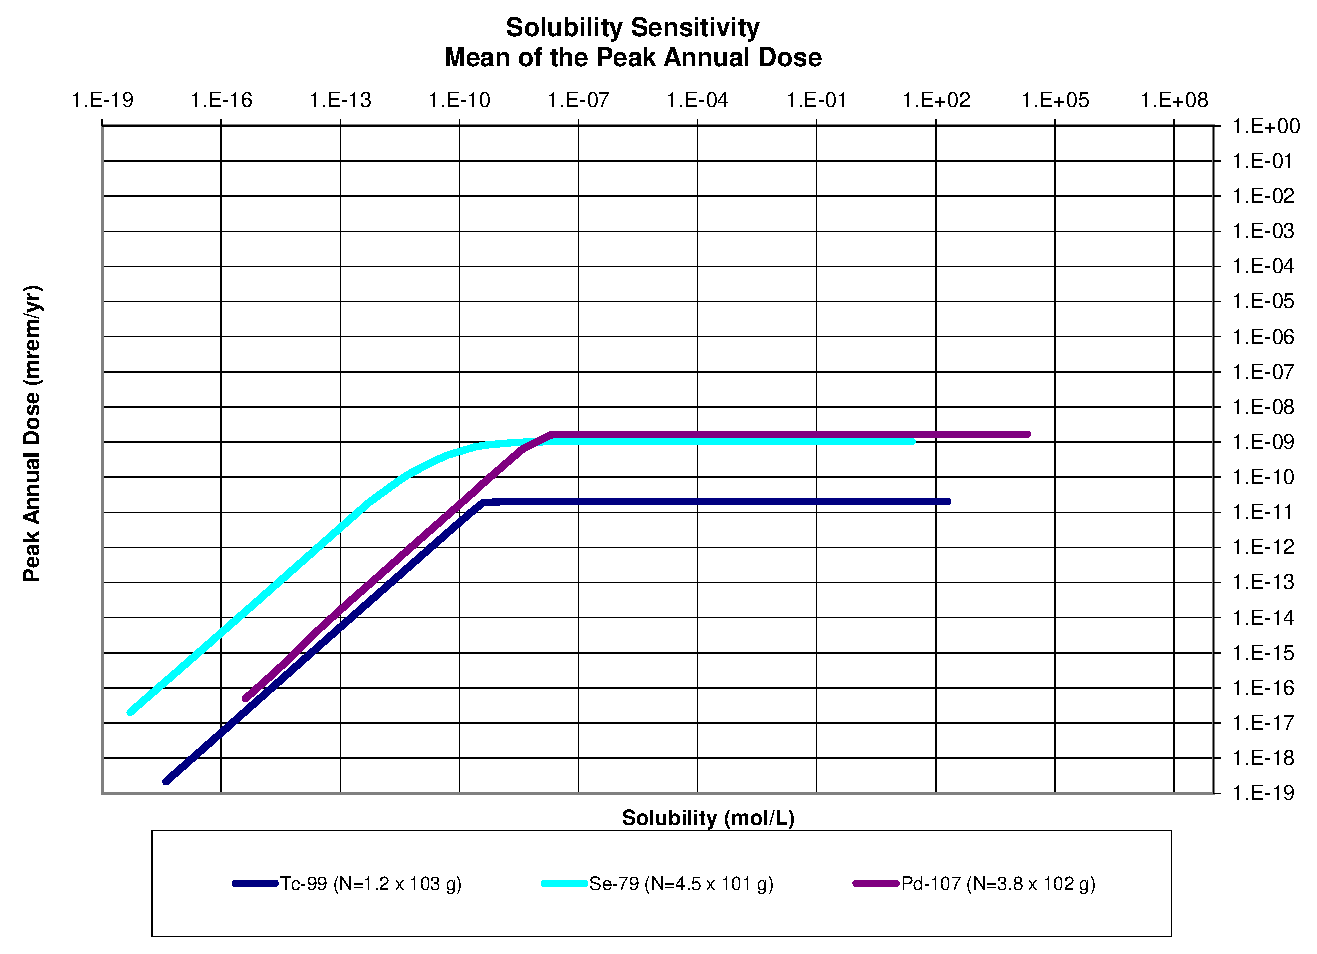
\includegraphics[width=0.7\linewidth]{./nuclide_demonstration/Solubility_Summary_Sol.eps}
\caption{Solubility limit sensitivity. The peak annual dose due to an inventory, 
$N$, of each isotope.}
\label{fig:SolSum}
\end{figure}
\end{frame}

In the parametric analysis of \Cyder performance, it was shown that the 
solubility sensitivity behavior closely matched that of the \gls{GDSM} 
sensitivity behaviors. Specifically, in Figure \ref{fig:sol}.

\begin{figure}[htbp!]
\begin{center}
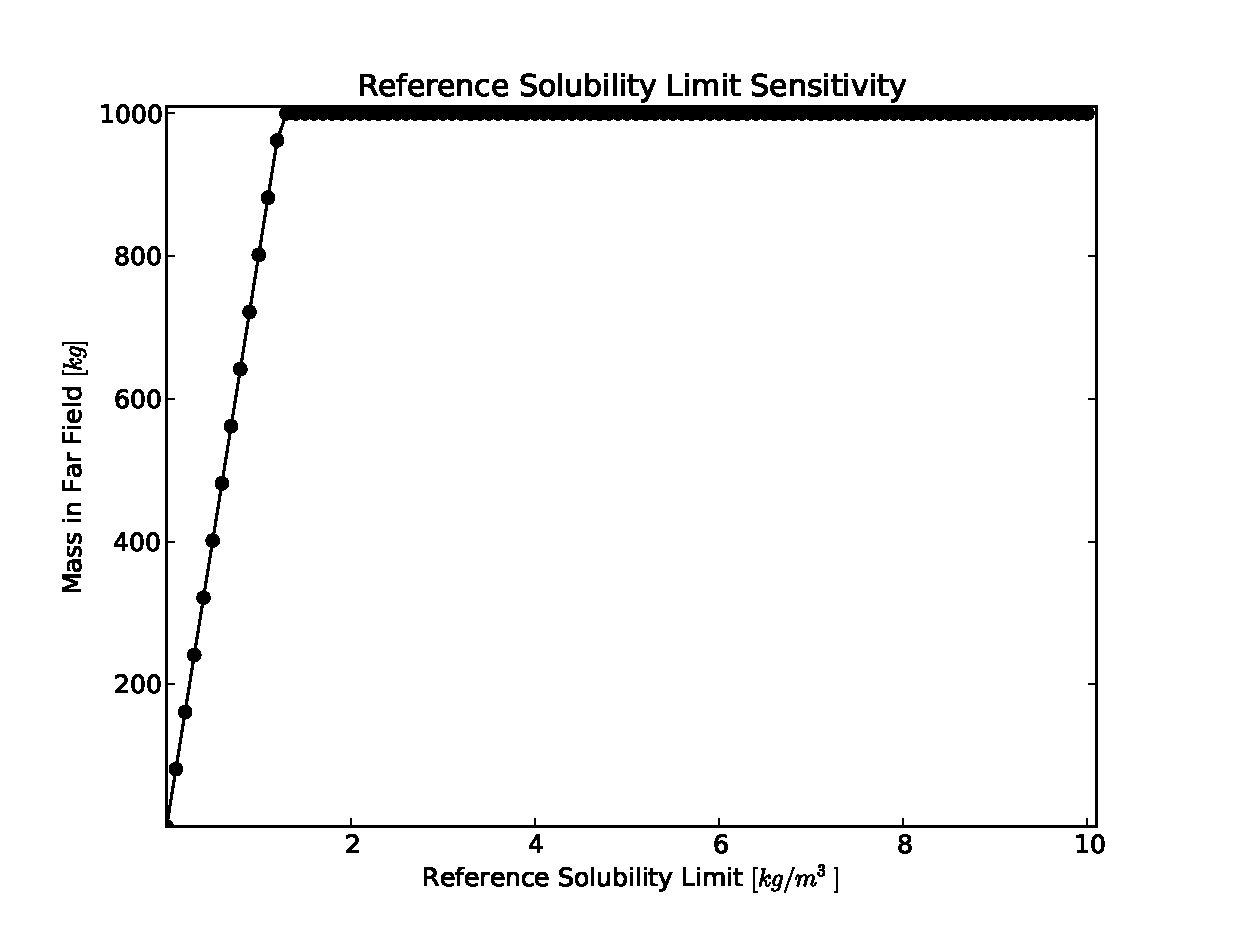
\includegraphics[width=0.8\textwidth]{./chapters/demonstration/bench/sol.eps}
\end{center}
\caption{Sensitivity demonstration of solubility limitation in Cyder for an 
arbitrary isotope assigned a variable solubility limit. }
\label{fig:sol_result}
\end{figure}



\end{frame}

\begin{frame}[ctb!]
\frametitle{Cyder Advective Diffusive Threshold}

\begin{frame}[ctb!]
\frametitle{Clay GDSM Sorption Sensitivity}
\begin{figure}[ht]
\centering
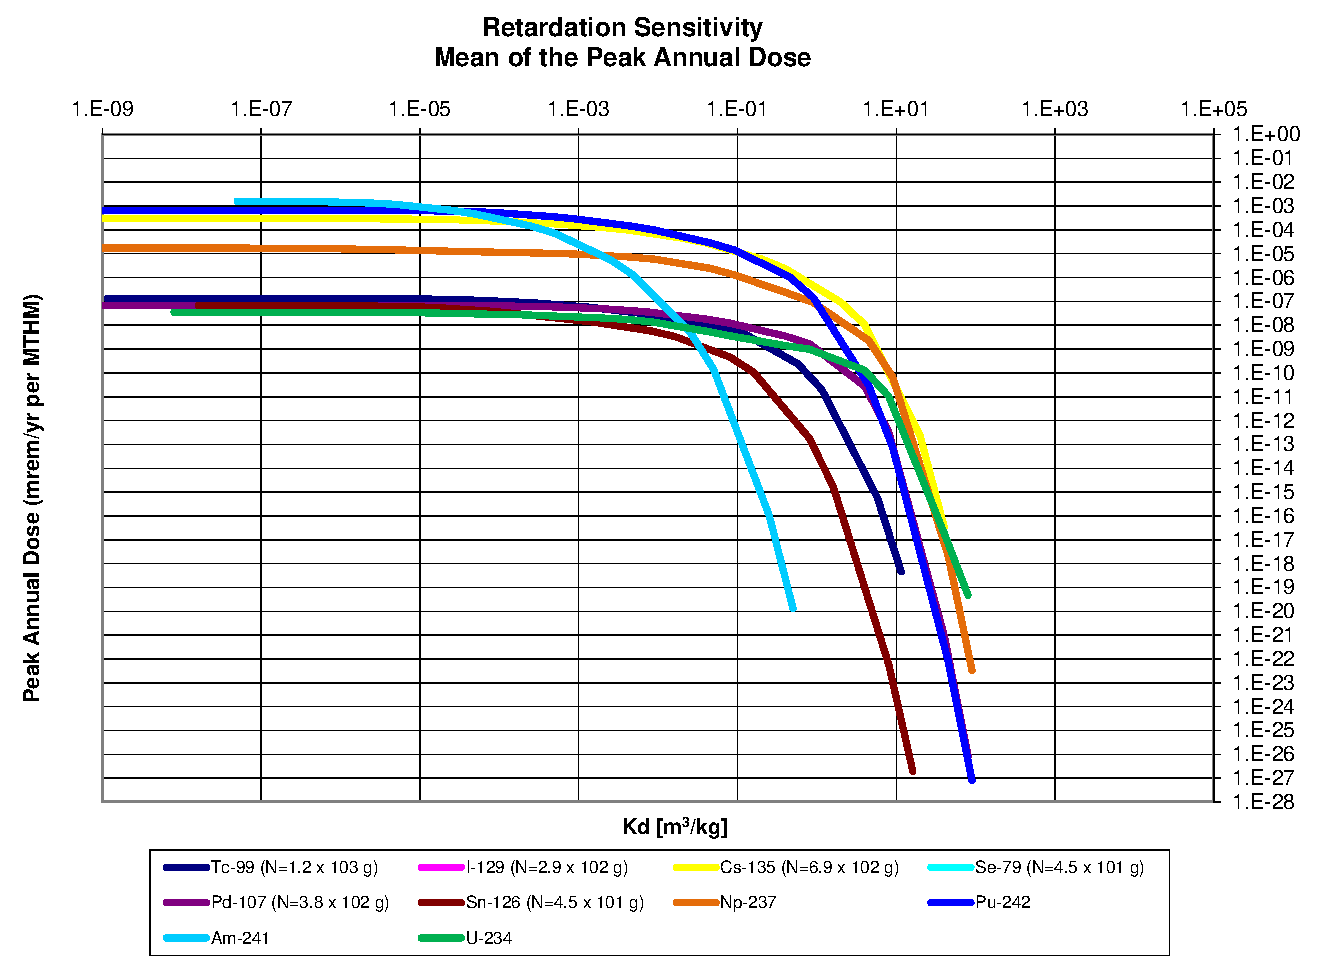
\includegraphics[width=0.7\linewidth]{./nuclide_demonstration/Retardation_Summary_kd.eps}
\caption{$K_d$ sensitivity.  The peak annual dose due to an inventory, 
$N$, of each isotope.}
\label{fig:KdSum}
\end{figure}

\end{frame}


\end{frame}

\begin{frame}[ctb!]
\frametitle{Cyder Advective Diffusive Threshold}
\begin{frame}[ctb!]
\frametitle{Clay GDSM Degradation Rate Sensitivity}

\begin{figure}[ht!]
\begin{minipage}[b]{0.45\linewidth}
\centering
\includegraphics[width=\linewidth]{./nuclide_demonstration/DegRate/I-129.eps}
\caption{$^{129}I$ waste form degradation rate sensitivity.}
\label{fig:WFDegI129}

\end{minipage}
\hspace{0.05\linewidth}
\begin{minipage}[b]{0.45\linewidth}

\includegraphics[width=\linewidth]{./nuclide_demonstration/DegRate/I-129-MF.eps}
\caption{$^{129}I$ inventory multiplier sensitivity.}
\label{fig:WFDegI129MF}

\end{minipage}
\end{figure}
\end{frame}

\begin{frame}[ctb]
\frametitle{Cyder Degradation Rate Sensitivity}
In the parametric sensitivity analysis conducted with the \Cyder tool, waste 
form degradation rate sensitvity similarly shows the two regimes noted in the 
GDSM analysis.  


\begin{figure}[htbp!]
\begin{center}
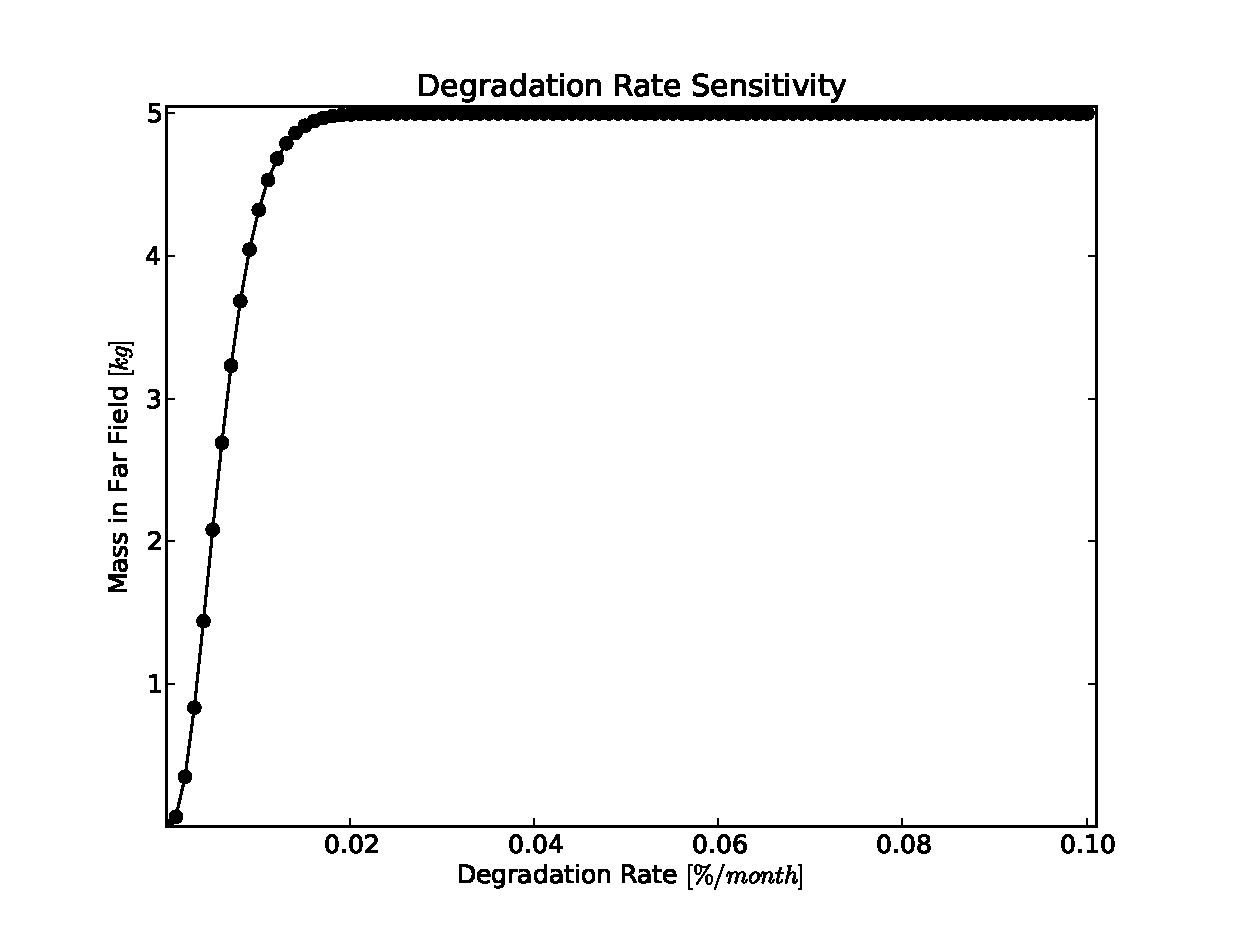
\includegraphics[width=0.7\linewidth]{./nuclide_demonstration/deg.eps}
\end{center}
\caption{Sensitivity demonstration of the degradation rate in \Cyder for an 
arbitrary isotope.}
\label{fig:deg}
\end{figure}
\end{frame}


%\subsection{Case IVI : Waste Package Failure Time and Diffusion Coefficient Sensitivity}
%\subsubsection{Waste Package Failure Time Sensitivity}

In the parametric sensitivity analysis discussed in Section 
\ref{sec:wpfail}, it was shown that For the clay repository, the waste 
package failure time is entirely irrelevant until waste package failure times 
reach the million or ten million year time scale. 

\begin{figure}[ht!]
  \centering
  \begin{minipage}[b]{0.45\linewidth}
    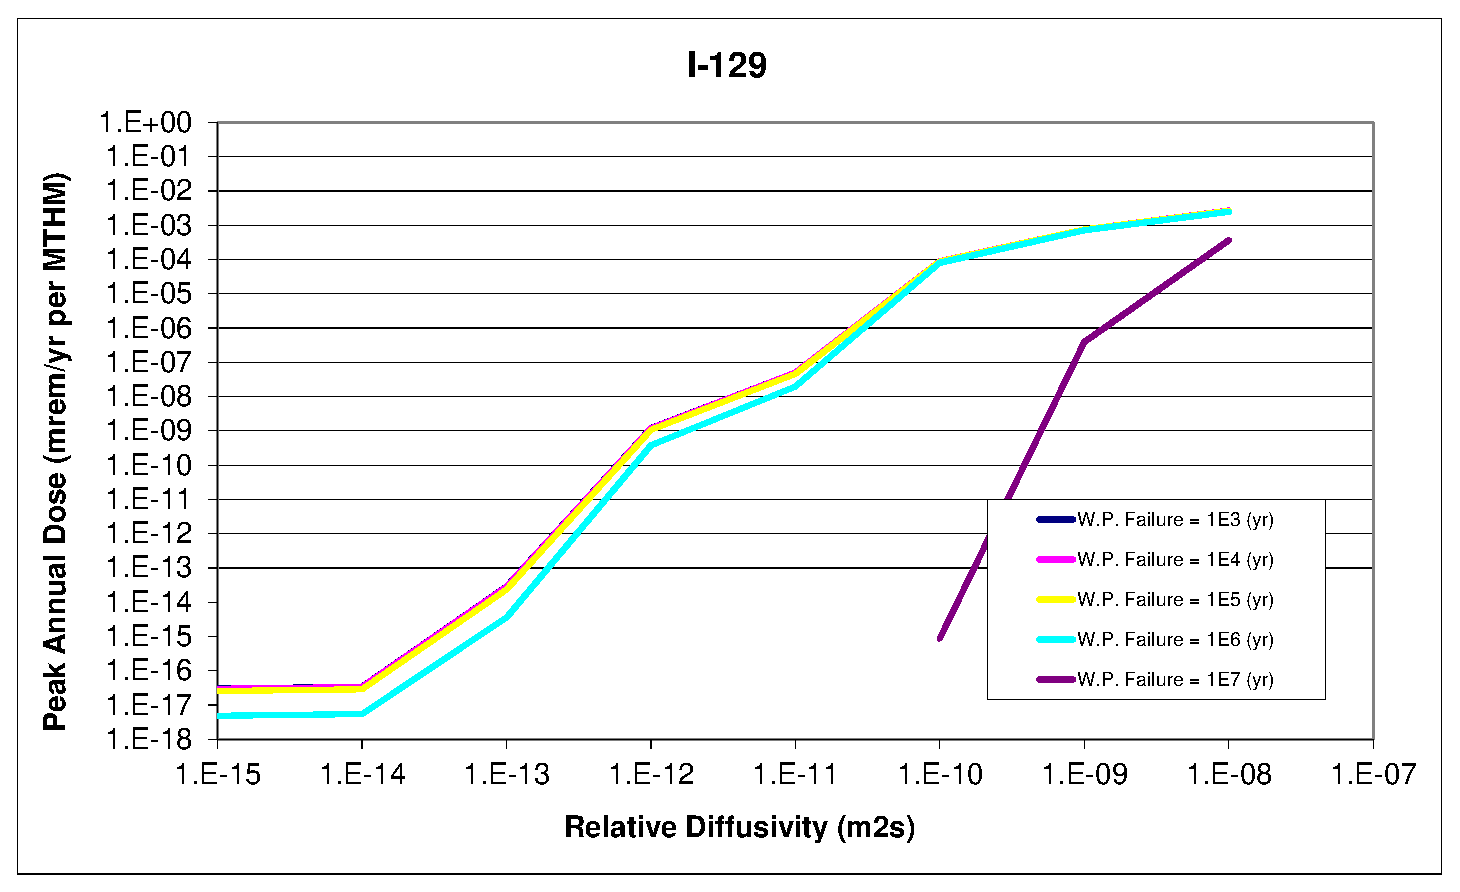
\includegraphics[width=\linewidth]{./chapters/nuclide_sensitivity/clay/WPFailExtended/I-129.eps}
    \caption{$^{129}I$ waste package failure time sensitivity. }
    \label{fig:WPFailI129}

  \end{minipage}
  \hspace{0.05\linewidth}
  \begin{minipage}[b]{0.45\linewidth}

    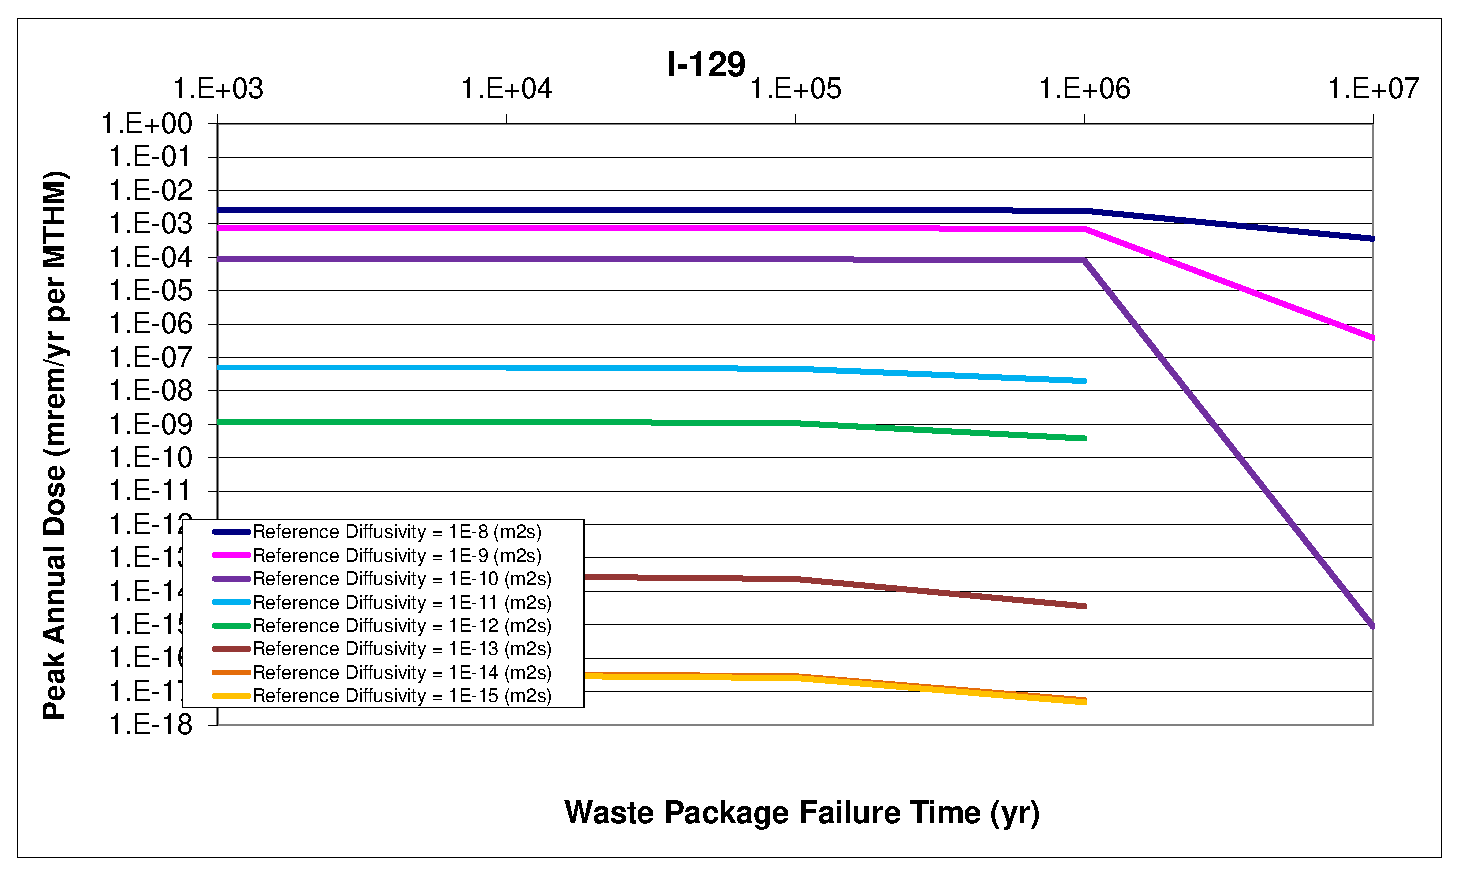
\includegraphics[width=\linewidth]{./chapters/nuclide_sensitivity/clay/WPFailExtended/I-129-WPFail.eps}
    \caption{$^{129}I$ waste package failure time sensitivity. }
    \label{fig:WPFailI129}

  \end{minipage}
\end{figure}
\begin{figure}[ht]
  \begin{minipage}[b]{0.45\linewidth}

    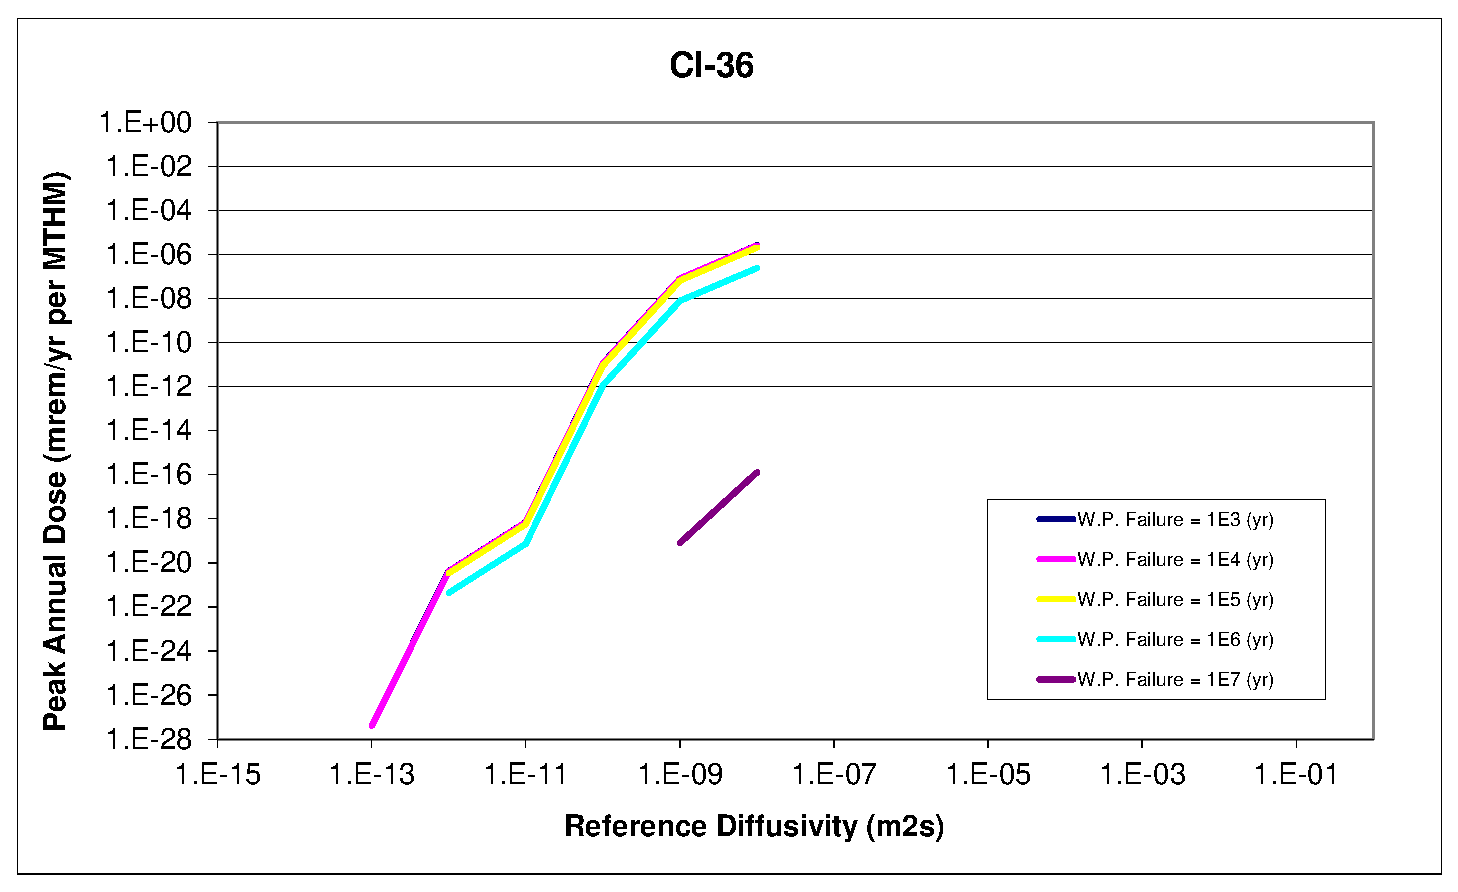
\includegraphics[width=\linewidth]{./chapters/nuclide_sensitivity/clay/WPFailExtended/Cl-36.eps}
    \caption{$^{36}Cl$ waste package failure time sensitivity. }
    \label{fig:WPFailCl36}

  \end{minipage}
  \hspace{0.05\linewidth}
  \begin{minipage}[b]{0.45\linewidth}

    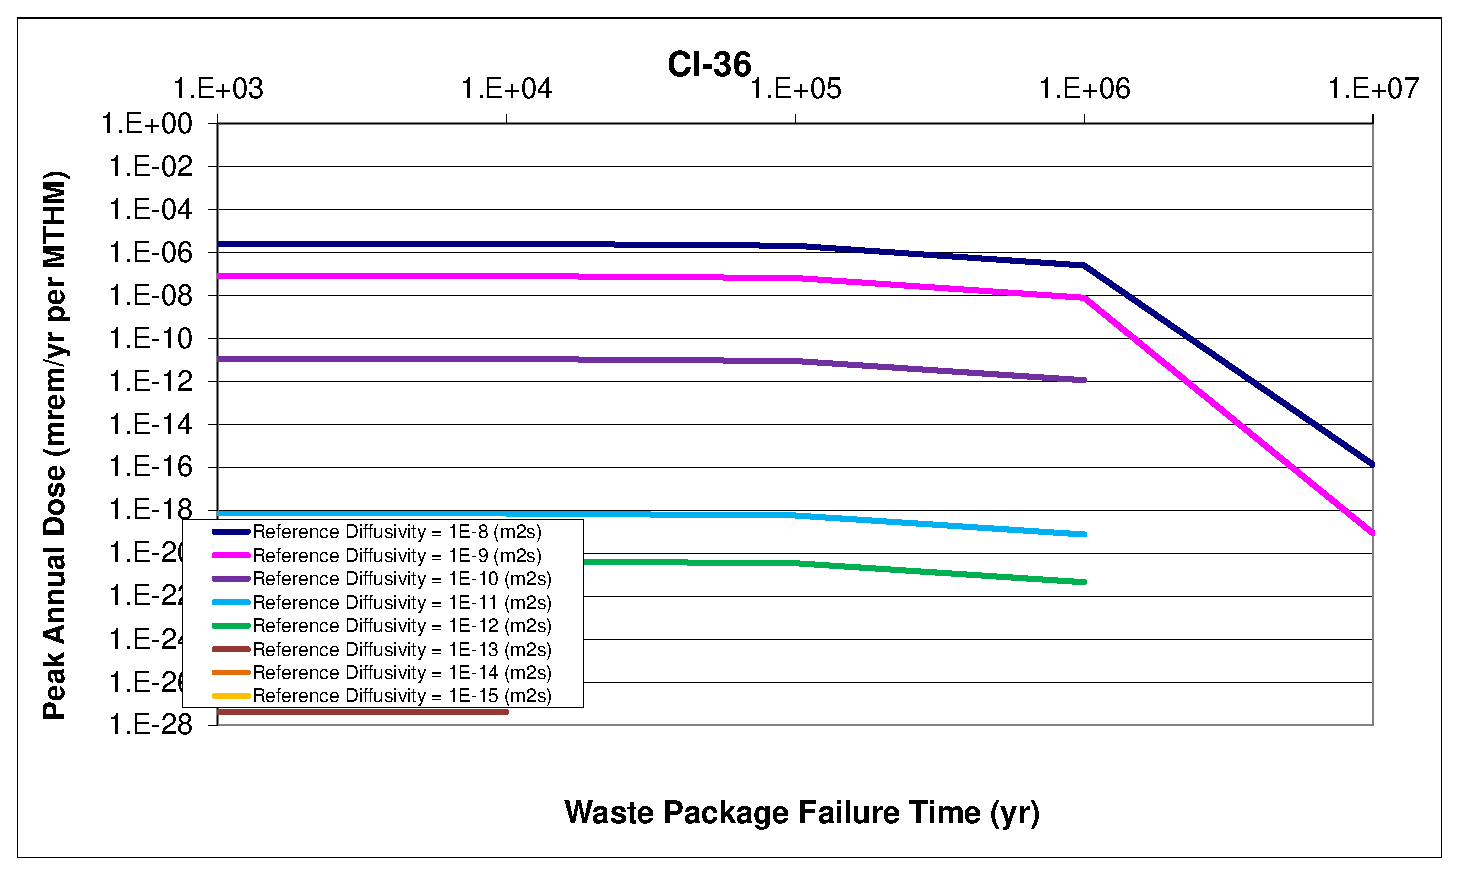
\includegraphics[width=\linewidth]{./chapters/nuclide_sensitivity/clay/WPFailExtended/Cl-36-WPFail.eps}
    \caption{$^{36}Cl$ waste package failure time sensitivity. }
    \label{fig:WPFailPuDaughters}

  \end{minipage}
\end{figure}


\begin{figure}[ht!]
  \centering
  \begin{minipage}[b]{0.45\linewidth}

    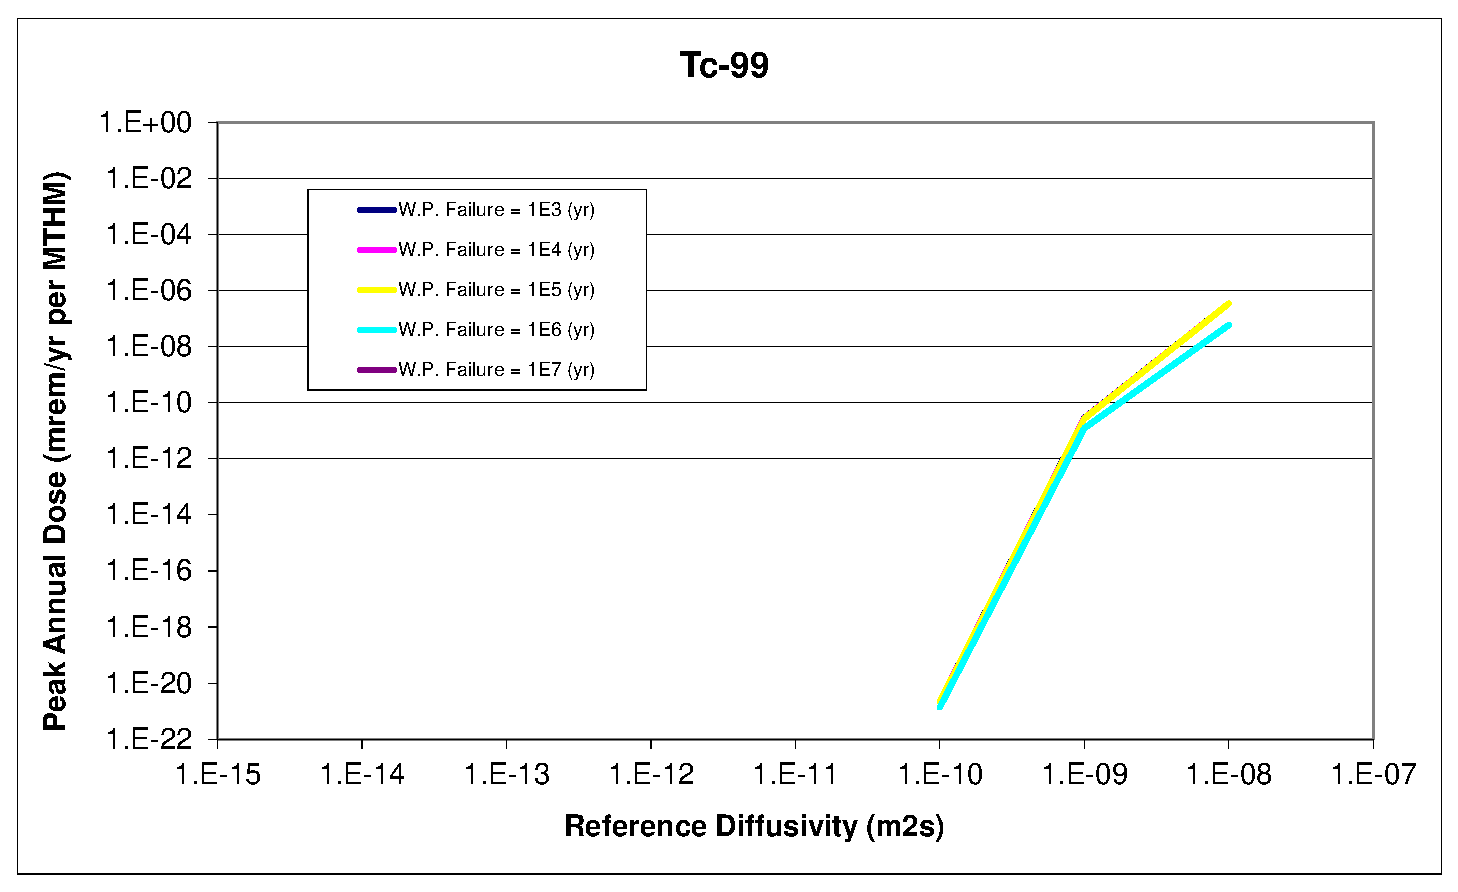
\includegraphics[width=\linewidth]{./chapters/nuclide_sensitivity/clay/WPFailExtended/Tc-99.eps}
    \caption{$^{99}Tc$ waste package failure time sensitivity. }
    \label{fig:WPFailTc99}

  \end{minipage}
  \hspace{0.05\linewidth}
  \begin{minipage}[b]{0.45\linewidth}

    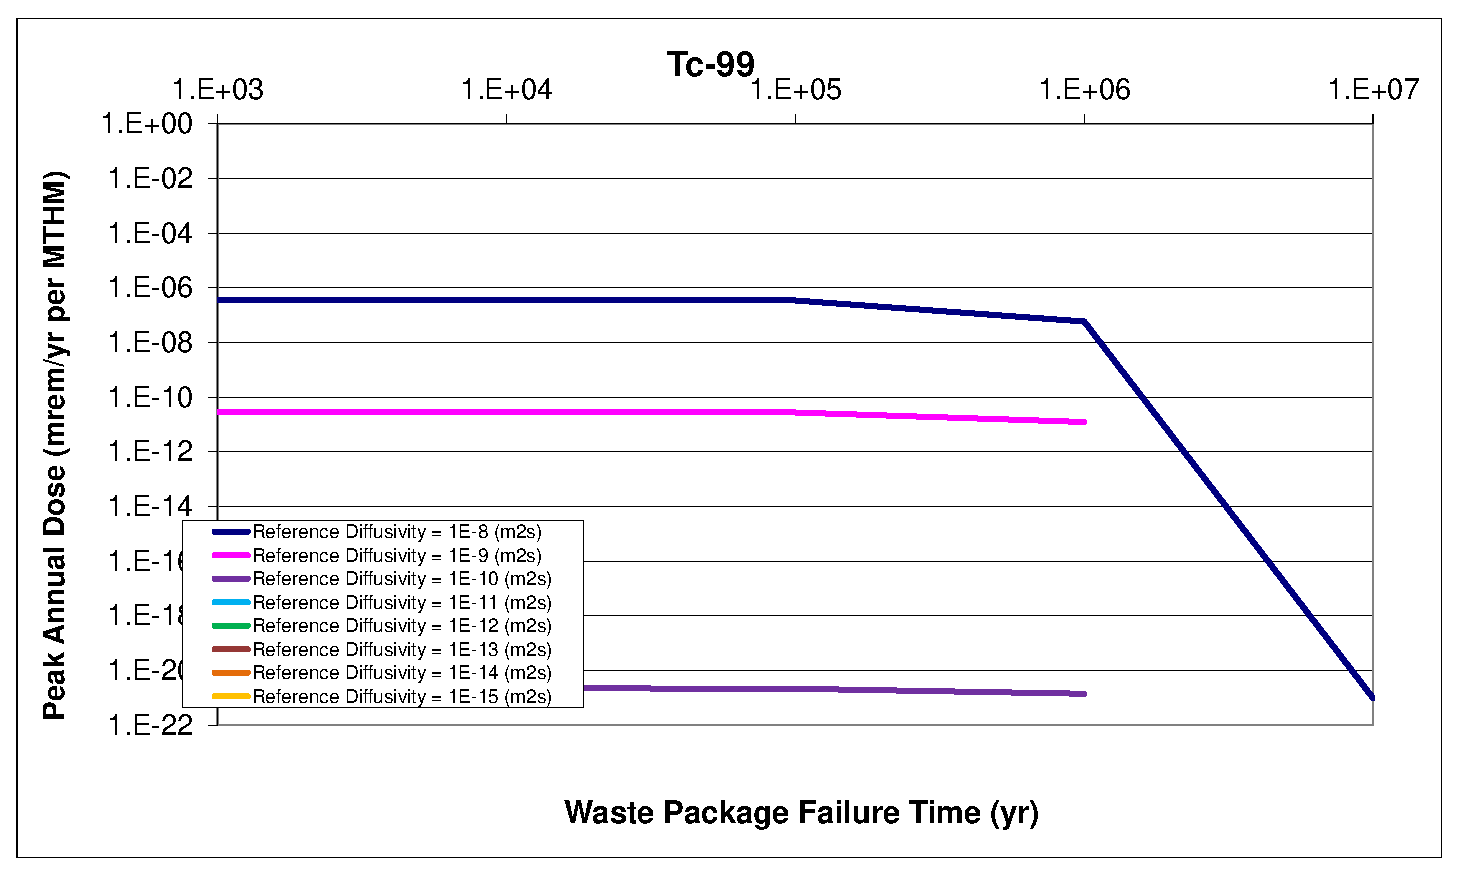
\includegraphics[width=\linewidth]{./chapters/nuclide_sensitivity/clay/WPFailExtended/Tc-99-WPFail.eps}
    \caption{$^{99}Tc$ waste package failure time sensitivity. }
    \label{fig:WPFailTc99}

  \end{minipage}
\end{figure}
\begin{figure}[ht]
  \begin{minipage}[b]{0.45\linewidth}

    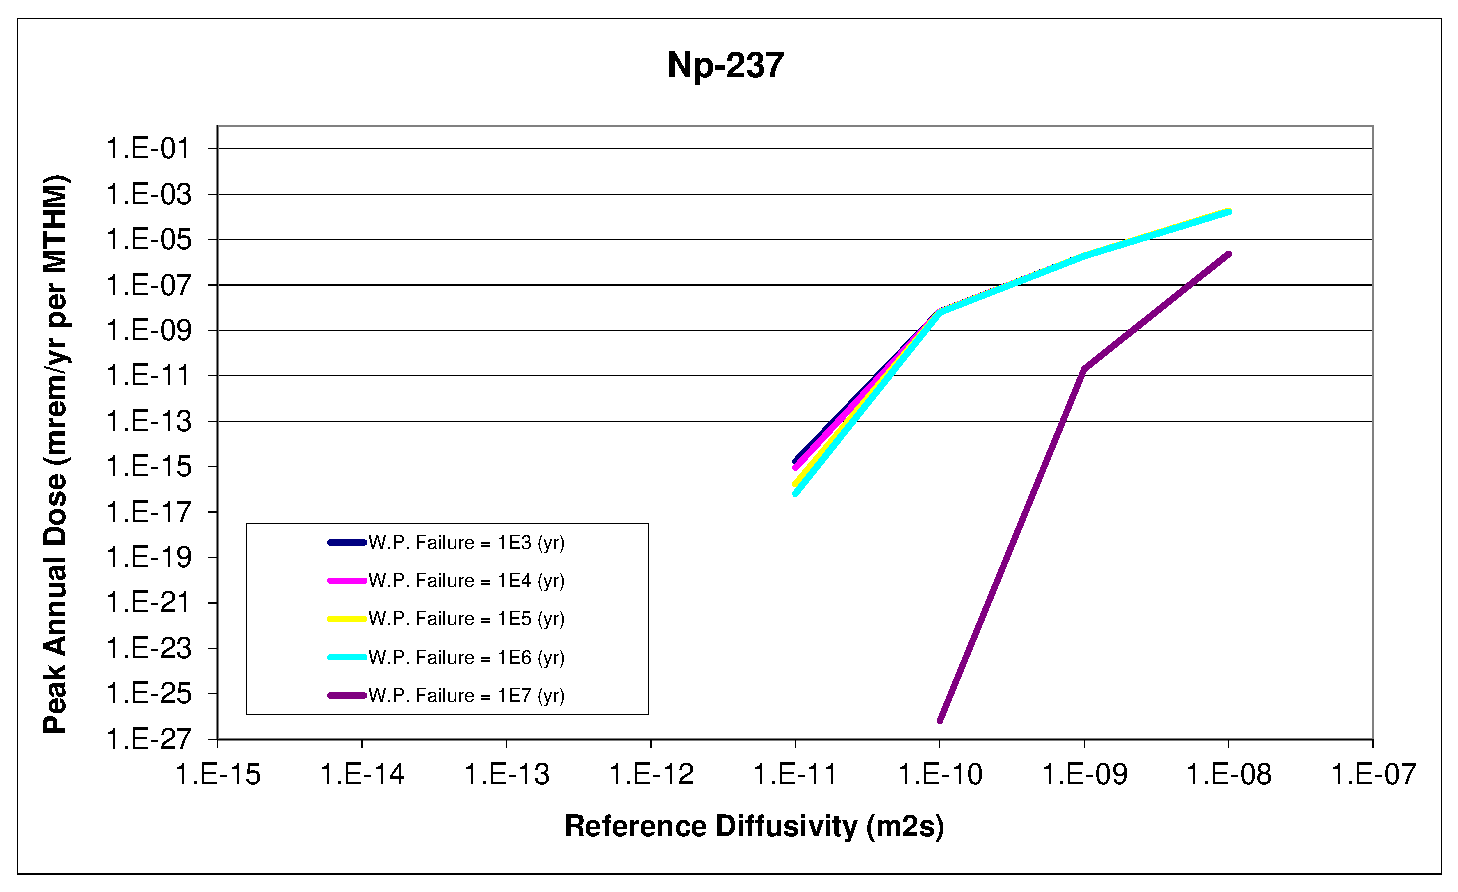
\includegraphics[width=\linewidth]{./chapters/nuclide_sensitivity/clay/WPFailExtended/Np-237.eps}
    \caption{$^{237}Np$ waste package failure time sensitivity. }
    \label{fig:WPFailNp237}

  \end{minipage}
  \hspace{0.05\linewidth}
  \begin{minipage}[b]{0.45\linewidth}

    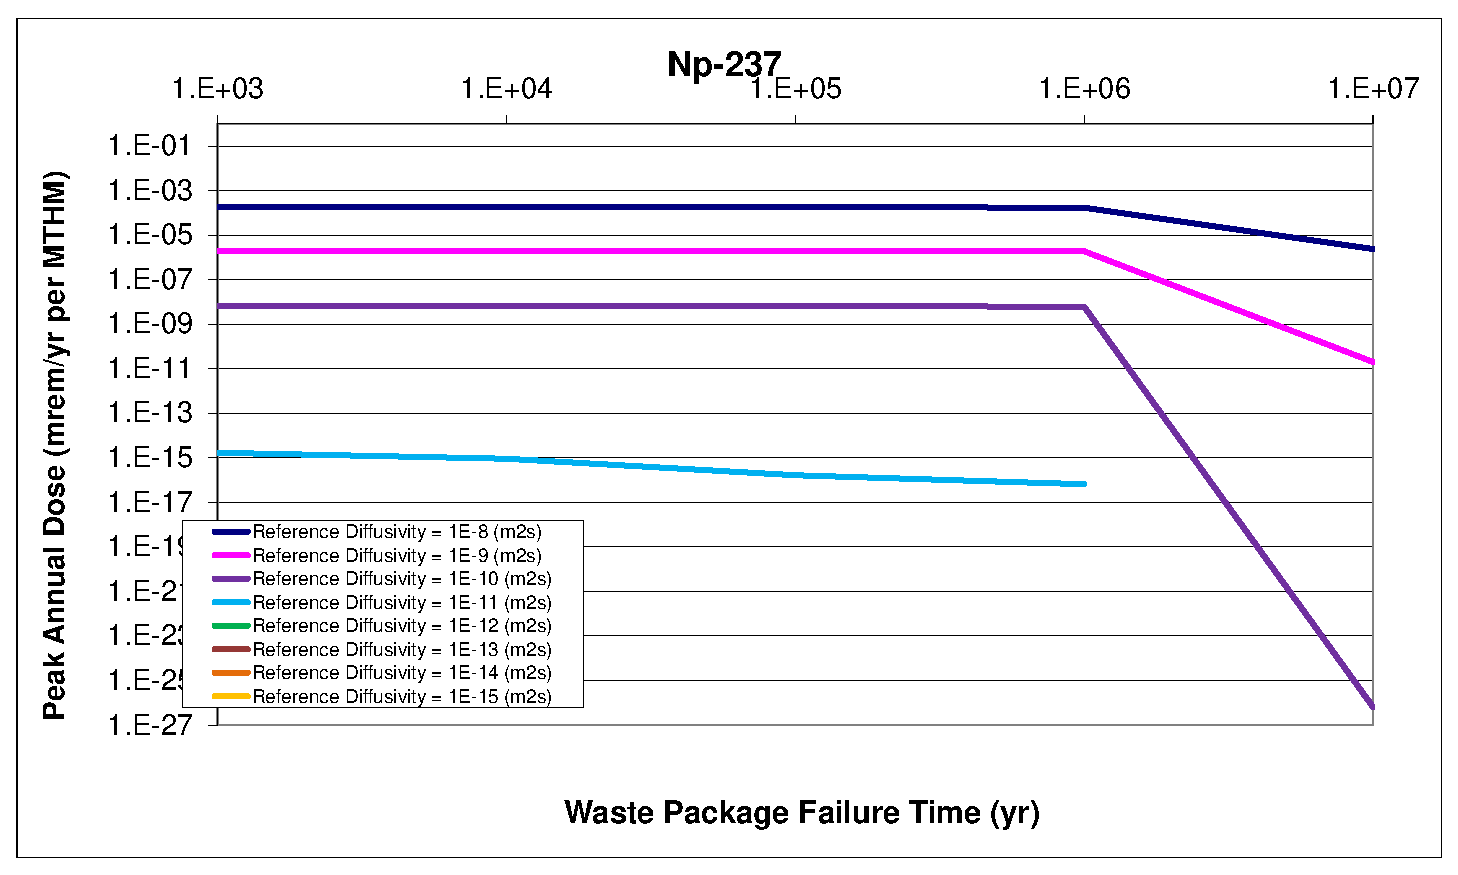
\includegraphics[width=\linewidth]{./chapters/nuclide_sensitivity/clay/WPFailExtended/Np-237-WPFail.eps}
    \caption{$^{237}Np$ waste package failure time sensitivity. }
    \label{fig:WPFailPuDaughters}

  \end{minipage}
\end{figure}

\clearpage



\end{frame}

\begin{frame}[ctb!]
\frametitle{Cyder Advective Diffusive Threshold}


\begin{frame}[ctb!]
\frametitle{GDSM Model Advective Diffusive Sensitivity}

\begin{figure}[htp!]
\begin{minipage}[b]{0.45\linewidth}
\centering
\includegraphics[width=\linewidth]{./nuclide_demonstration/AdvVelDiff/I-129.eps}
\caption{$^{129}I$ reference diffusivity sensitivity.}
\label{fig:VAdvVelI129}

\end{minipage}
\hspace{0.05\linewidth}
\begin{minipage}[b]{0.45\linewidth}

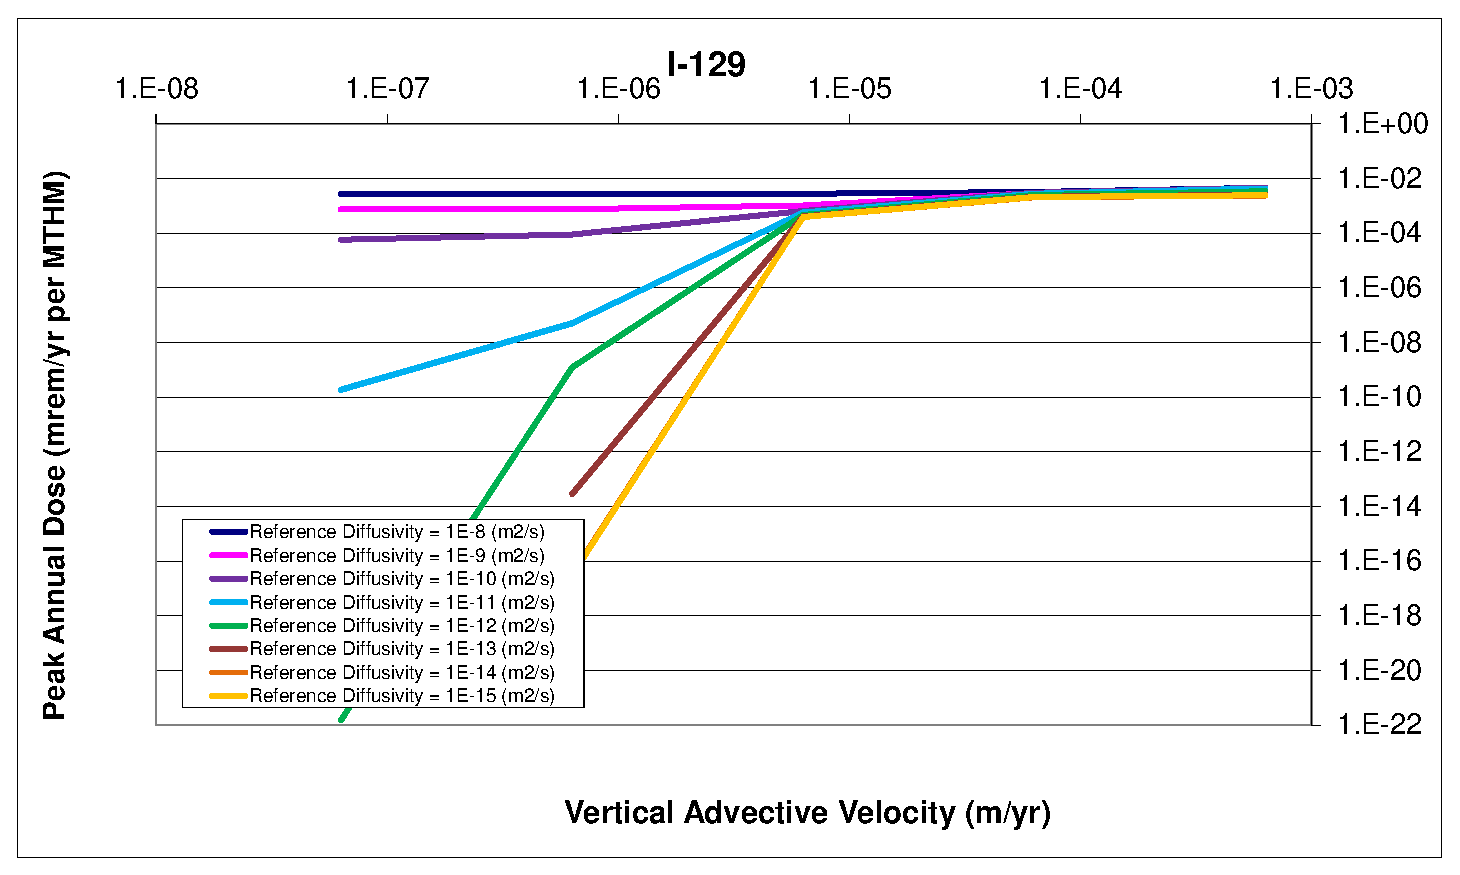
\includegraphics[width=\linewidth]{./nuclide_demonstration/AdvVelDiff/I-129-VAdvVel.eps}
\caption{$^{129}I$ vertical advective velocity sensitivity.}
\label{fig:VAdvVelI129VAdvVel}

\end{minipage}
\end{figure}
\end{frame}


\subsubsection{Advection vs. Diffusion Sensitivity Cyder Results}
Some of the  radionuclide transport models in \Cyder depend on the advective velocity as well as the diffusion 
characteristics of the medium. By evaluating the sensitivity to the advective velocity and reference 
diffusivity of the radionuclide transport in the MixedCell model, trends similar to those found in the \gls{GDSM} were found with the \Cyder tool. 
Specifically, increased advection and increased diffusion lead to greater release. Also, when both are varied, a boundary between diffusive and advective
regimes can be seen. An example of these results are shown in Figure \ref{fig:mixed_adv_diff}.
 
\begin{figure}[ht]
\centering
%\includegraphics[width=\linewidth]{./chapters/demonstration/bench/mixed_diff.eps}
\caption[Advection vs. Diffusion Sensitivity in Cyder]{Dual advective velocity 
and reference diffusivity sensitivity for a non-sorbing, infinitely soluble 
nuclide.}
\label{fig:mixed_adv_diff}
\end{figure}


\end{frame}

\section{Thermal Transport Validation}\label{sec:thermal_benchmarks}
The mass transfer interfaces between the mass balance models are essential to 
the understanding of the \Cyder paradigm.  

In groundwater transport, contaminants are transported by dispersion and 
advection. It is customary to define the combination of molecular diffusion and 
mechanical mixing as the dispersion tensor, $D$, such that, for a conservative 
solute (infinitely soluble and non-sorbing), the mass conservation equation 
becomes \cite{schwartz_fundamentals_2004, wang_introduction_1982, 
van_genuchten_analytical_1982}:

     \begin{align}
      J &= J_{dis} + J_{adv}\nonumber
      \intertext{where}
      J_{dis} &= \mbox{ Total Dispersive Mass Flux }[kg/m^2/s]\nonumber\\
      &= -\theta(D_{mdis} + \tau D_m)\nabla C \nonumber\\ 
      &= -\theta D\nabla C \nonumber\\
      J_{adv} &= \mbox{ Advective Mass Flux }[kg/m^2/s]\nonumber\\
      &= \theta vC\nonumber\\
      \tau &= \mbox{ Tortuosity }[-] \nonumber\\
      \theta &= \mbox{ Porosity }[-] \nonumber\\
      D_m &= \mbox{ Molecular diffusion coefficient }[m^2/s]\nonumber\\
      D_{mdis} &= \mbox{ Coefficient of mechanical dispersivity}[m^2/s]\nonumber\\
      D &= \mbox{ Effective Dispersion Coefficient }[m^2/s]\nonumber\\
      C &= \mbox{ Concentration }[kg/m^3]\nonumber\\
      v &= \mbox{ Fluid Velocity in the medium }[m/s].\nonumber
    \end{align}

For uniform flow in $\hat{k}$, 
    \begin{align}
      J &=\left(-\theta D_{xx} \frac{\partial C}{\partial x}
             \right)\hat{\imath}
             + \left( -\theta D_{yy} \frac{\partial C}{\partial y}
            \right)\hat{\jmath}
            + \left( -\theta D_{zz} \frac{\partial C}{\partial z}
             + \theta v_zC 
            \right)\hat{k}.
      \label{unidirflow}
    \end{align}

Solutions to this equation can be categorized by their boundary conditions.  
Those boundary conditions serve as the interfaces between components in the 
\Cyder library of nuclide transport models by way of advective, dispersive, 
coupled, and fixed fluxes.  This is supported by implementation in which 
vertical advective velocity is uniform throughout the system and in which 
parameters such as the dispersion coefficient are known for each component. 


<pphw>

  introduce 2 different mass transfer modes

  explicit: a model is chosen to represent the mass transfer and the sink 
  inventory is updated based on this transfer rate (I think these are only used 
  between a pair of 0-D models [KDH note: all components allow this on their 
  external boundary. Only the 0D models also allow this on their inner 
  boundary.]) introduce overall concept of combined advective and diffusive mass transfer

  implicit: a sink inventory is updated based on its distribution model, and 
  mass is transferred to accomplish the change in inventory


\section{Waste Package Spacing Sensitivity Study}\label{sec:spacing}
The waste package spacing, $s$ of geologic repository concept effects the areal 
decay heat burden in the repository and has a strong effect on the thermal 
energy deposited per unit area in the medium. 

In the creation of the \gls{STC} database, the waste package spacing was varied 
across a number of values for each isotope, $i$, limiting 
radius $r_{calc}$, thermal diffusivity $\alpha_{th}$, and thermal conductivity $K_{th}$, considered.  By 
varying the waste package spacing of the repository model from $0.1-5 [m]$
this sensitivity analysis succeeds in capturing the domain of 
waste package spacings present in geologic repository concepts under 
consideration. 

\begin{figure}[htbp!]
\begin{center}
%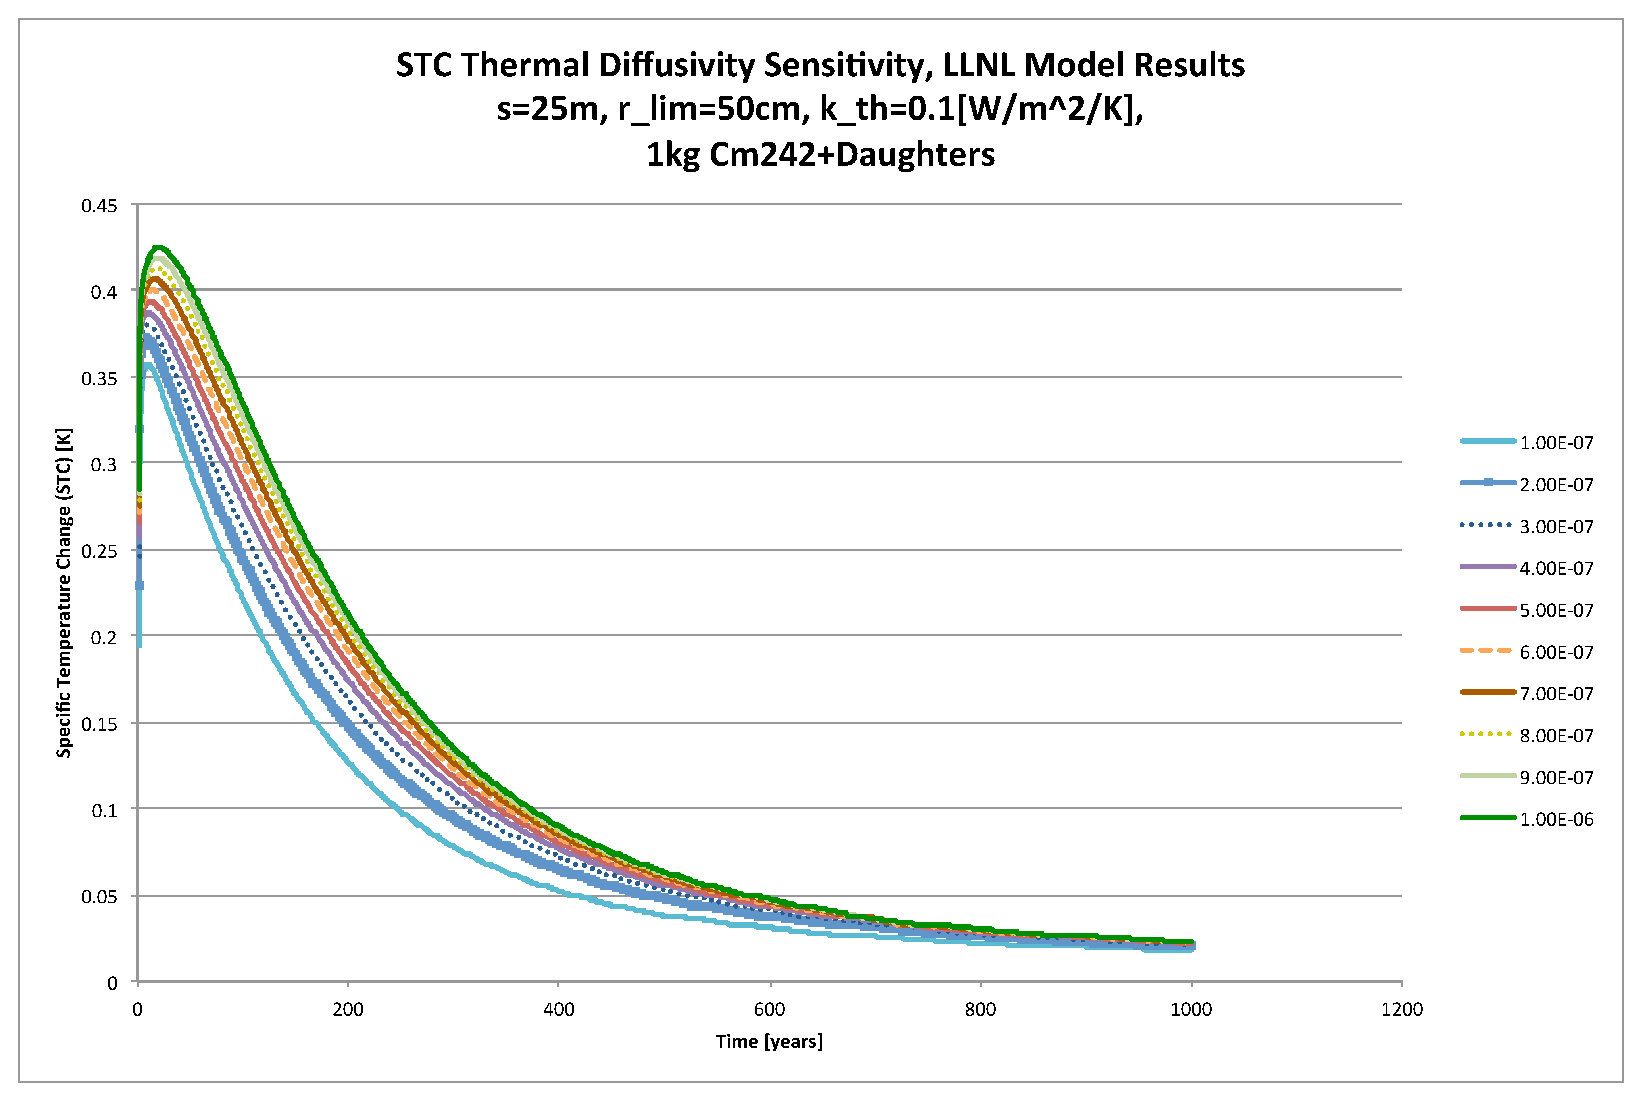
\includegraphics[width=0.7\textwidth]{./chapters/demonstration/diffusivity/Cm242alpha_kth_low.eps}
\end{center}
\caption[$K_{th}$ Sensitivity for Low $\alpha_{th}$]{Increased waste package 
spacing decreases areal thermal energy deposition 
(here represented by \gls{STC}) in the near field (here $r_{calc} = 0.5m$).}
\label{fig:Cm242alpha_kth_low}
\end{figure}

Figure \ref{fig:Cm242alpha_kth_low} shows the trend, visible for all isotopes, 
that increased waste package spacing of a medium decreases thermal energy 
deposition in the near field. This indicates that waste package spacing is 
an important parameter for repository concept design.





\begin{frame}[ctb!]
\frametitle{LLNL Model Thermal Conductivity Sensitivity}
By varying the thermal conductivity of the repository model from 0.1 to 4.5 
$[W\cdot m^{-1} \cdot K^{-1}]$, this sensitivity analysis succeeds in capturing 
the domain of thermal conductivities witnessed in high thermal conductivity 
salt deposits as well as low thermal conductivity clays.


\begin{figure}[htbp!]
\begin{center}
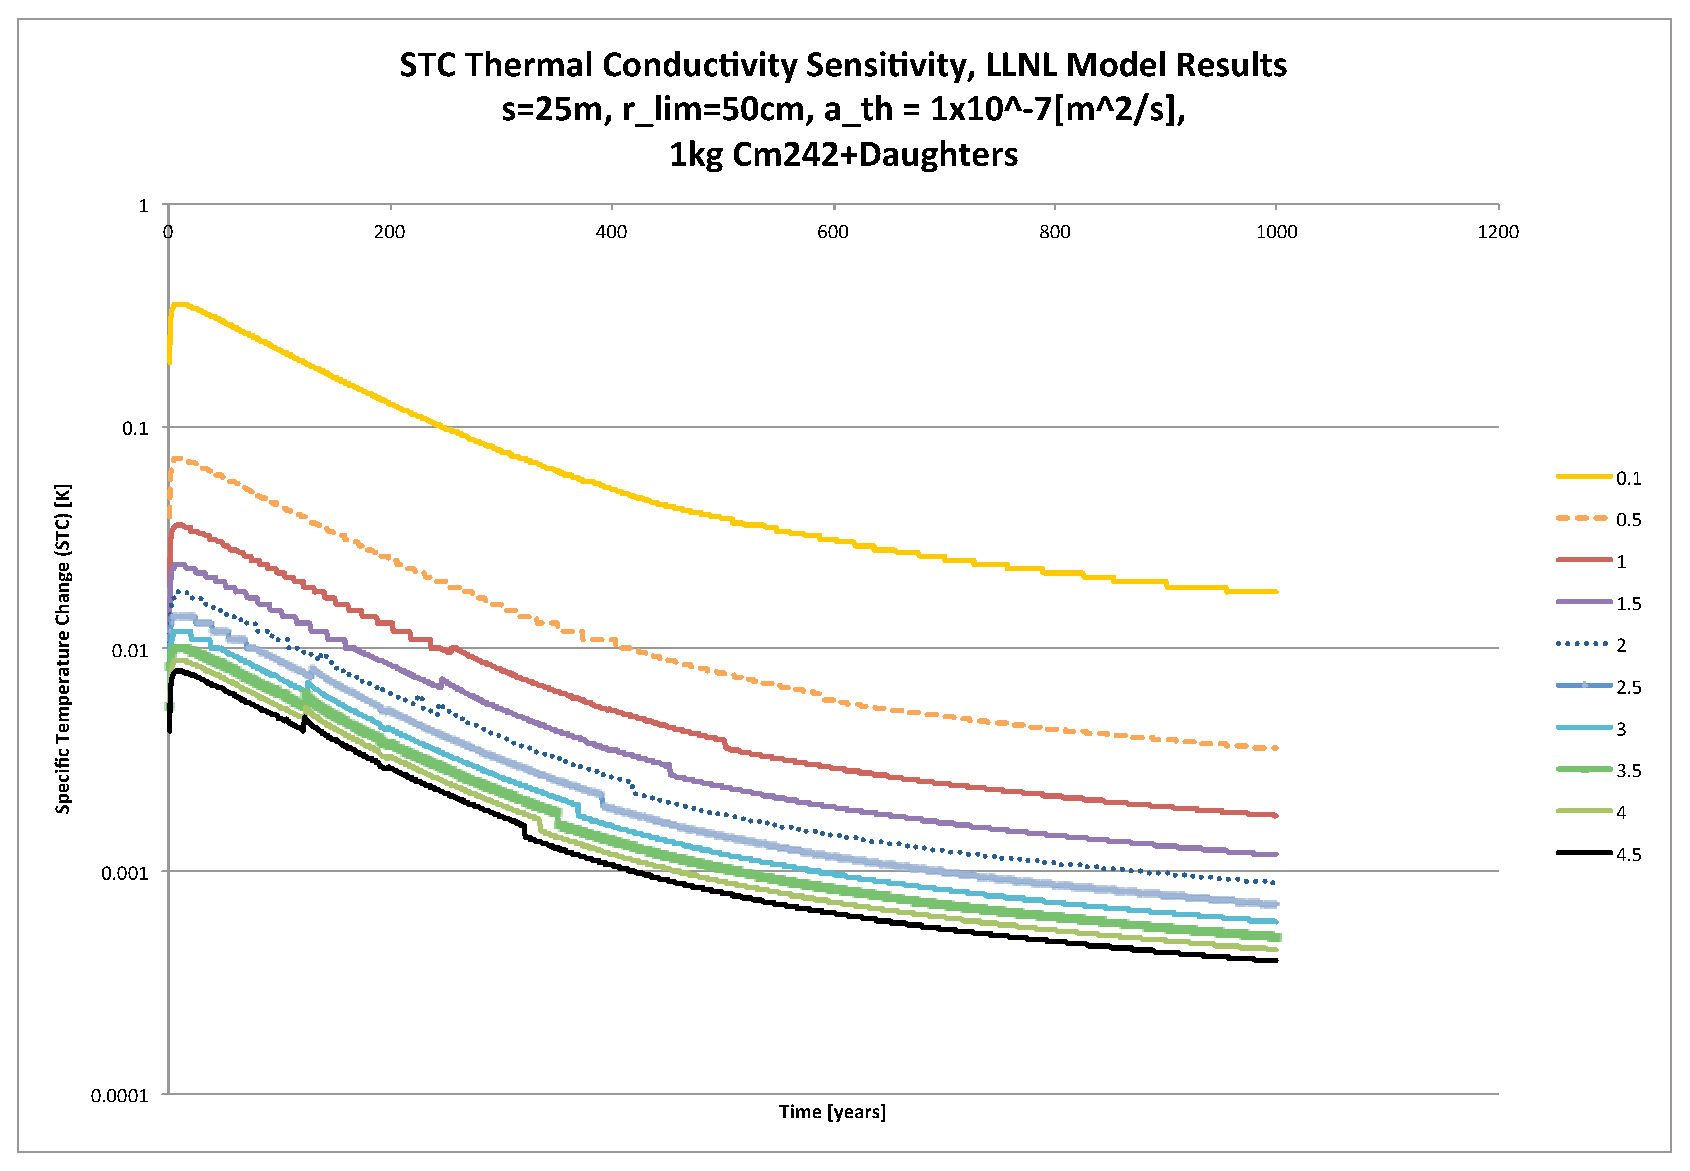
\includegraphics[height=0.7\textheight]{./thermal_demonstration/conductivity/Cm242kth_alpha_low.eps}
\end{center}
\caption[$K_{th}$ Sensitivity for Low $\alpha_{th}$ in LLNL Model]{Increased thermal conductivity decreases thermal energy deposition 
(here represented by STC) in the near field (here $r_{calc} = 0.5m$).}
\label{fig:Cm242Kth_alpha_low}
\end{figure}

\end{frame}


\begin{frame}[ctb!]
\frametitle{Cyder Thermal Conductivity and Limiting Radius Sensitivity}

Figures \ref{fig:kr} and \ref{fig:ks} validate the trend noted above that 
increased thermal conductivity of a medium decreases thermal energy deposition 
in the near field. Additionally, analysis with the \Cyder STC database 
demonstrates the way in which the importance of spacing and the importance of 
the limiting radius decrease with increasing $K_{th}$.

\begin{figure}[htbp!]
\begin{center}
\includegraphics[height=0.7\textheight]{./thermal_demonstration/conductivity/kr.eps}
\end{center}
\caption[$K_{th}$ vs. $r_{lim}$ Sensitivity in Cyder]
{Cyder results agree with 
those of the LLNL model. The importance of the limiting radius decreases with 
increased $K_{th}$. The above example thermal profile results from 10kg of 
$^{242}Cm$}
\label{fig:kr}
\end{figure}
\end{frame}

\begin{frame}[ctb!]
\frametitle{Cyder Thermal Conductivity and Limiting Radius Sensitivity}

\begin{figure}[htbp!]
\begin{center}
\includegraphics[height=0.7\textheight]{./thermal_demonstration/conductivity/ks.eps}
\end{center}
\caption[$K_{th}$ vs. Waste Package Spacing Sensitivity in Cyder]{Cyder results agree with 
those of the LLNL model. The importance of the limiting radius decreases with 
increased $K_{th}$. The above example thermal profile results from 10kg of 
$^{242}Cm$}
\label{fig:ks}
\end{figure}
\end{frame}




\subsection{Diffusion Coefficient of Far Field}
\label{sec:diffusivity}

In clay media, diffusion dominates far field hydrogeologic transport due to 
characteristically low hydraulic head gradients and permeability. Thus, the effective diffusion 
coefficient is a parameter to which repository performance in clay media is 
expected to be very sensitive. 

The sensitivity of the peak dose to the reference diffusivity of the 
host rock was analyzed.  In this model, the reference diffusivity of the medium 
was the input parameter used to vary the effective diffusivity in a controlled 
manner. In GoldSim's transport module, the effective diffusion coefficient is 
defined as 

\begin{align}\label{diffcoeff}
  D_{eff} &= n\tau D_{ref}D_{rel} \\ % ?  
       D_{eff} &= ~~\mbox{effective diffusion coefficient }[m^2/s],\nonumber\\
       D_{rel} &= ~~\mbox{relative diffusivity for each isotope in water }[\%],\nonumber\\
       D_{ref} &= ~~\mbox{reference diffusivity in water }[m^2/s],\nonumber\\
       \tau &= ~~\mbox{tortuosity} [\%], \nonumber \\ 
       n &= ~~\mbox{porosity}[\%].\nonumber\\
  \label{GDSEdiff}
\end{align}

The reference diffusivity was altered while the porosity and the tortuosity 
were both set to 1. Thus, the simulation rendered the effective diffusivity 
equal to the product of the reference diffusivity and the relative diffusivity 
(set to 1 for all isotopes).  This allowed the diffusivity to be controlled 
directly for all isotopes.

The waste inventory total mass was also altered for each value of the reference 
diffusivity.  That is, the radionuclide inventory in a reference 
\gls{MTHM} of commercial spent nuclear fuel was multiplied by a scalar mass factor.  
It was expected that changing these two parameters in tandem would capture the 
importance of diffusivity in the far field to the repository performance 
as well as a threshold at which the effect of waste inventory dissolution is 
attenuated by solubility limits.

Finally, in order to isolate the effect of the far field behavior, the waste form 
degradation rate was set to be very high as were the solubility and advective 
flow rate through the  \gls{EBS}. This guaranteed that contaminant flowthrough 
in the near field was unhindered, leaving the far field as the dominant barrier 
to release.


\subsubsection{Parametric Range}
\label{sec:diffCoeffRange}

The forty runs corresponded to eight values of relative diffusivity and five 
values of inventory mass multiplier. That is, the reference diffusivity was varied over the 
eight magnitudes between $ 10^{-8}$ and $10^{-15}$ $[m^2 /s]$ . 
The Mass Factor, the unitless inventory multiplier, was simultaneously varied over 
the five magnitudes between $10^{-4}$ and $10^{1} [-]$. That is, the 
radionuclide inventory was varied between $10^{-4}$ and $10^{1}$ of that in one 
\gls{MTHM} of \gls{SNF}, which is expected to cover the full range of 
inventories in current wasteforms.

\begin{table}[hbp!]
\centering
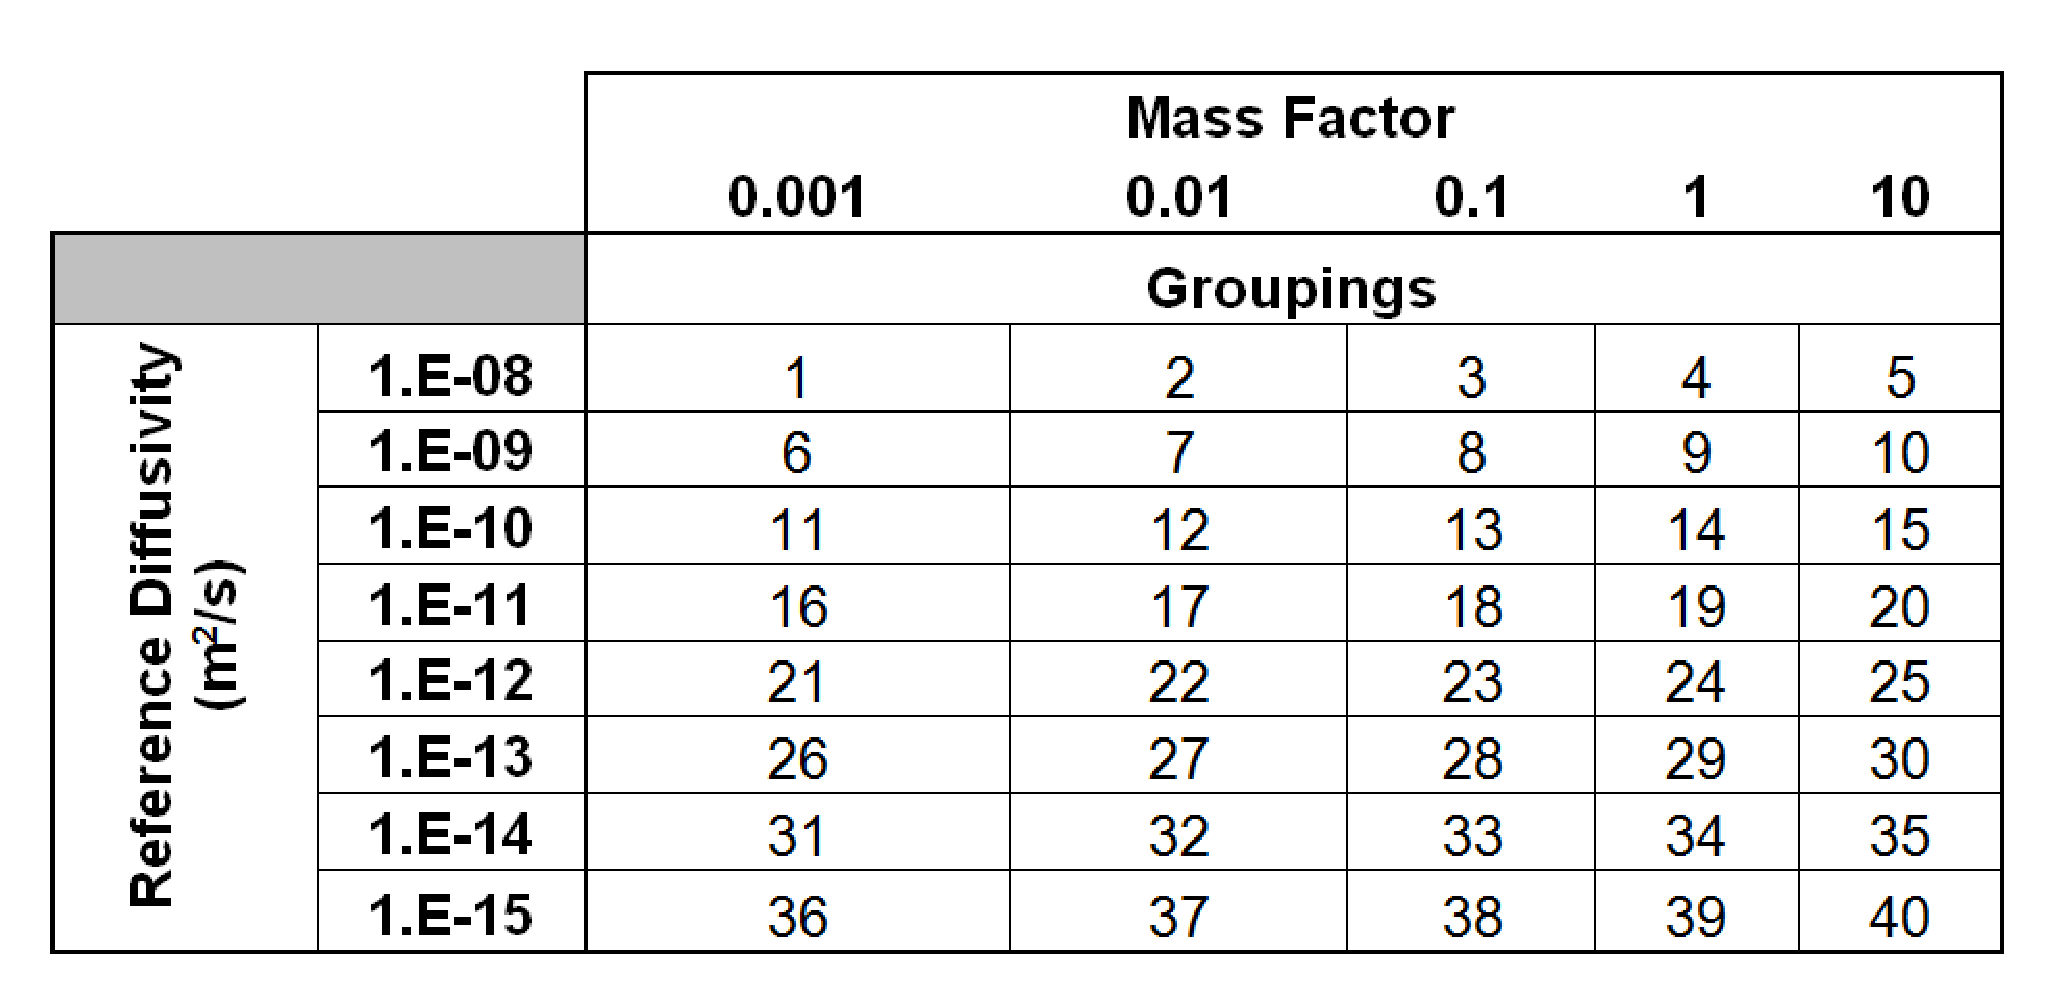
\includegraphics[width=0.7\textwidth]{./chapters/nuclide_sensitivity/clay/DiffCoeffAndInvEBSFail/DiffCoeffAndInvGroups.eps}
\caption{Diffusion coefficient and mass factor simulation groupings.}
\label{tab:DiffCoeffAndInvGroups}
\end{table}

\subsubsection{Results}


The peak doses due to highly soluble, non-sorbing elements such as $I$ and $Cl$, 
are  proportional to the radionuclide inventory and 
largely directly proportional to the relative diffusivity. This can be seen for 
the cases of $^{129}I$ and $^{36}Cl$ in Figures \ref{fig:DCInvI129}, 
\ref{fig:DCInvI129MF}, \ref{fig:DCInvCl36} and \ref{fig:DCInvCl36MF}.

\begin{figure}[ht]
\centering
\includegraphics[width=\linewidth]{./chapters/nuclide_sensitivity/clay/DiffCoeffAndInvEBSFail/I-129.eps}
\caption{$^{129}I$ relative diffusivity sensitivity.}
\label{fig:DCInvI129}
\end{figure}

\begin{figure}[ht]
\centering
\includegraphics[width=\linewidth]{./chapters/nuclide_sensitivity/clay/DiffCoeffAndInvEBSFail/I-129-MF.eps}
\caption{$^{129}I$ mass factor sensitivity.}
\label{fig:DCInvI129MF}
\end{figure}

\begin{figure}[ht]
\centering
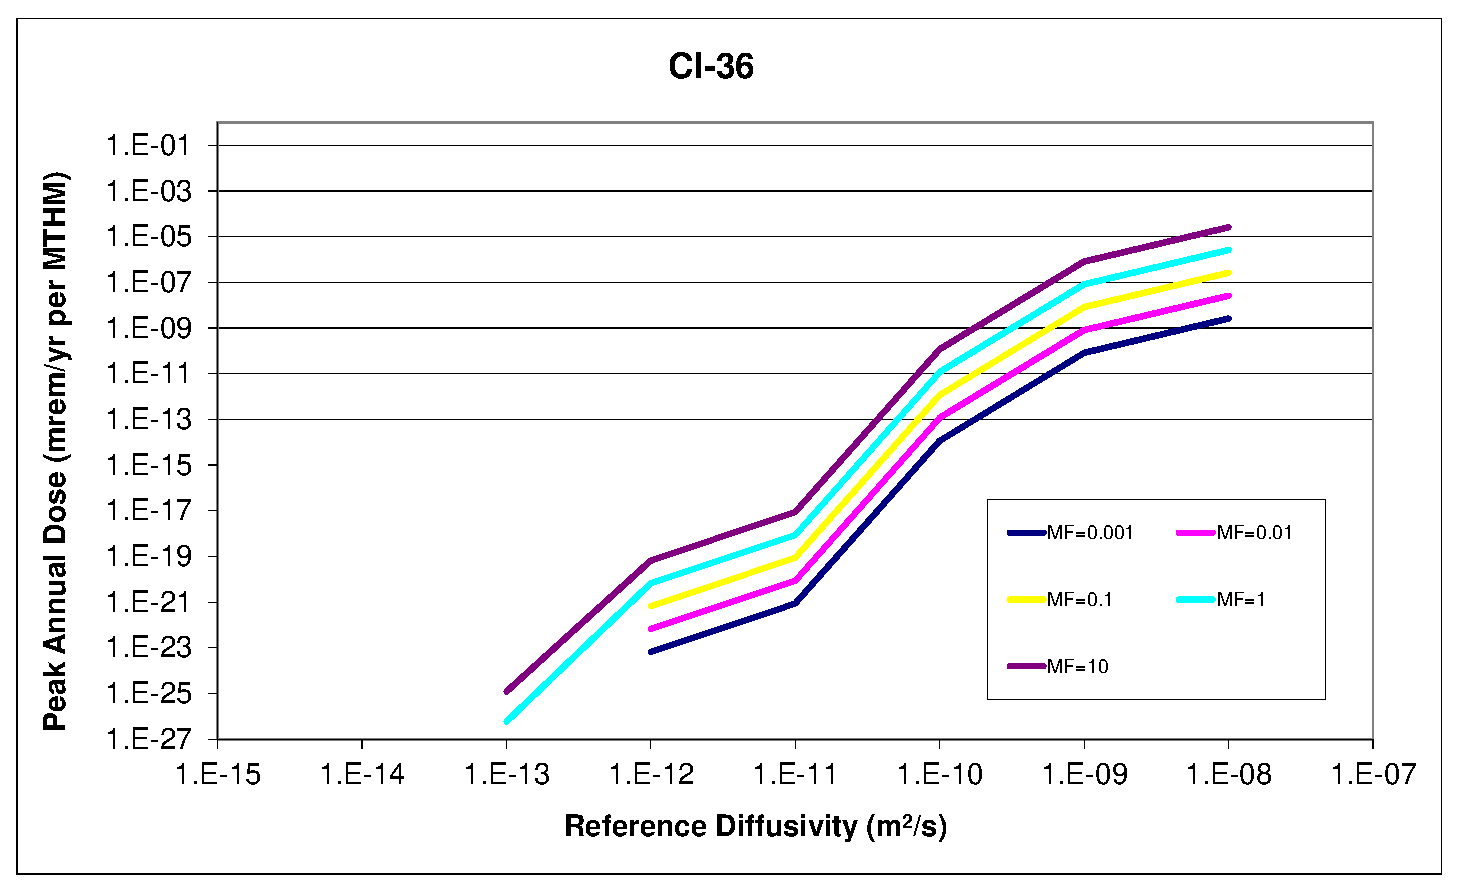
\includegraphics[width=\linewidth]{./chapters/nuclide_sensitivity/clay/DiffCoeffAndInvEBSFail/Cl-36.eps}
\caption{$^{36}Cl$ relative diffusivity sensitivity.}
\label{fig:DCInvCl36}
\end{figure}

\begin{figure}[ht]
\centering
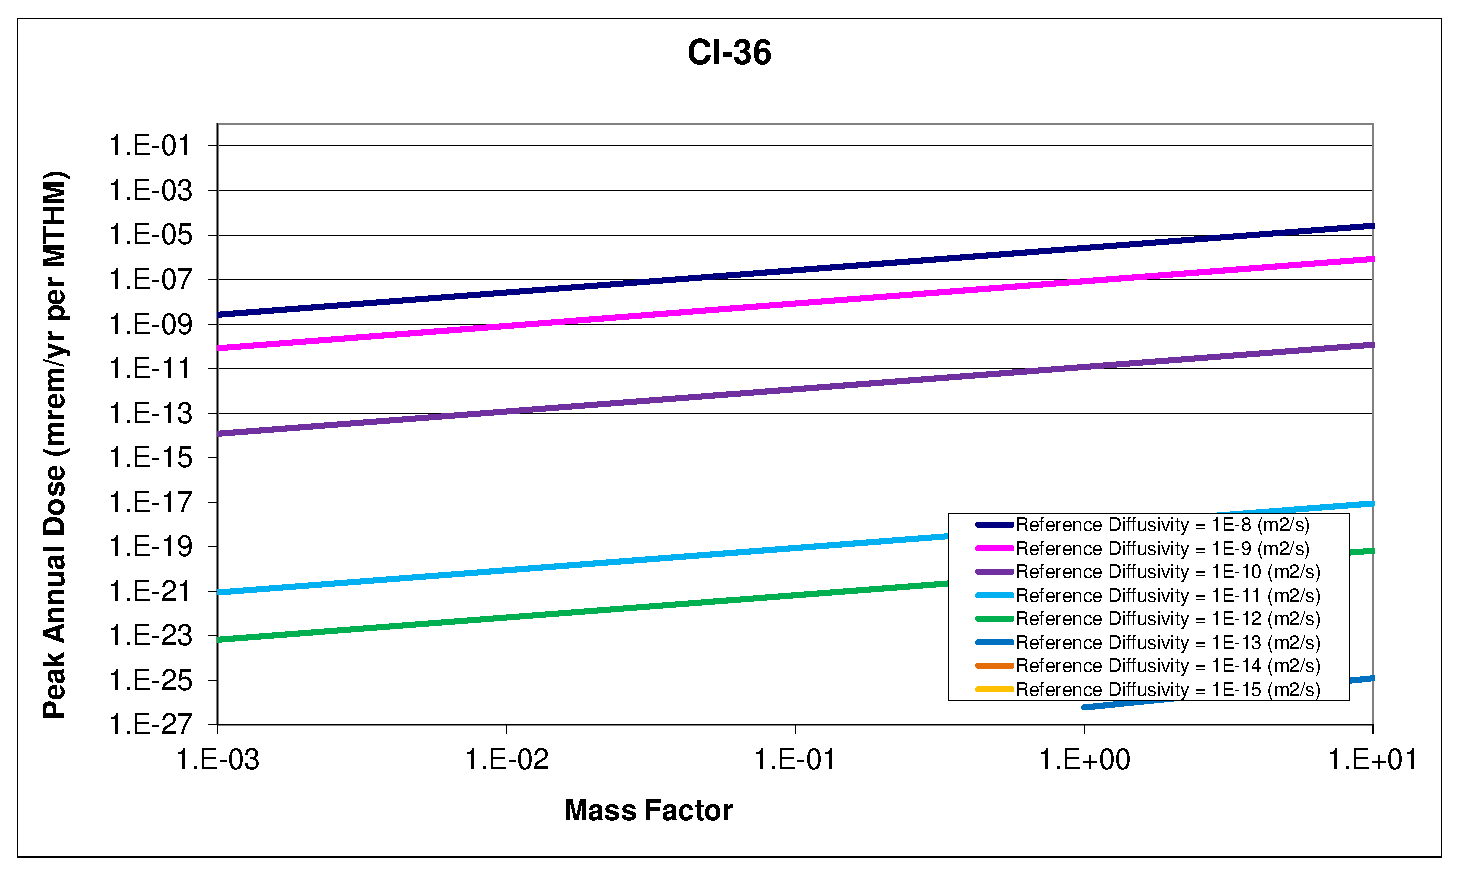
\includegraphics[width=\linewidth]{./chapters/nuclide_sensitivity/clay/DiffCoeffAndInvEBSFail/Cl-36-MF.eps}
\caption{$^{36}Cl$ mass factor sensitivity.}
\label{fig:DCInvCl36MF}
\end{figure}

Long lived $^{129}I$ and $^{36}Cl$ are assumed to have near complete solubility, 
so in Figures \ref{fig:DCInvI129} and \ref{fig:DCInvCl36}, the effect of a 
solubility limited attenuation regime is not seen. Even for very low 
diffusivities, the diffusion length of the far field is the primary barrier. In 
Figures \ref{fig:DCInvI129MF} and \ref{fig:DCInvCl36MF} it is clear that in the 
absence of solubility limitation and sorption, the peak dose is directly 
proportional to mass factor. 

Both $Cl$ and $I$ are soluble and non-sorbing. The amount of $^{129}I$ in the 
\gls{SNF} inventory is greater than the amount of $^{36}Cl$, so a difference in 
magnitudes are expected, however, the trends should be the same. Since the 
halflife of $^{36}Cl$, $3\times10^5[yr]$, is much shorter than the half life of 
$^{129}I$, $1.6\times10^7[yr]$, a stronger proportional dependence on mass 
factor is seen for $Cl$ due to its higher decay rate. 

With the exception of those dose-contributors assumed to be completely soluble, 
two regimes were visible in the results of this analysis. In low diffusion 
coefficient regime, the diffusive pathway through the homogeneous permeable 
porous medium in the far field continues to be a  dominant barrier to nuclide 
release for normal (non-intrusive) repository conditions. 

In the second regime, for very high diffusion coefficients, the effects of 
additional attenuation phenomena in the natural system can be seen.  The 
dependence of peak annual dose on mass factor was consistently directly 
proportional for all isotopic groups.

The peak doses due to solubility limited, sorbing elements such as $Np$ and 
$Tc$ demonstrate two major regimes. In the first regime, for 
low values of mass factor, the mean of the peak annual dose rates is directly 
proportional to both reference diffusivity and mass factor.  For higher values 
of mass factor, the sensitivity to reference diffusivity and mass factor are 
both attenuated at higher values.  The attenuation in these regimes 
is due to natural system attenuation, most notably, sorption.

$^{237}Np$ and $^{99}Tc$ exhibit a strong proportional relationship 
between diffusivity and dose in Figures \ref{fig:DCInvTc99} and 
\ref{fig:DCInvNp237}. This relationship is muted as diffusivity 
increases. Both are directly proportional to mass factor until they reach the 
point of attenuation by their solubility limits, as can be seen in 
Figures \ref{fig:DCInvTc99MF} and \ref{fig:DCInvNp237MF}.

\begin{figure}[ht!]
\centering
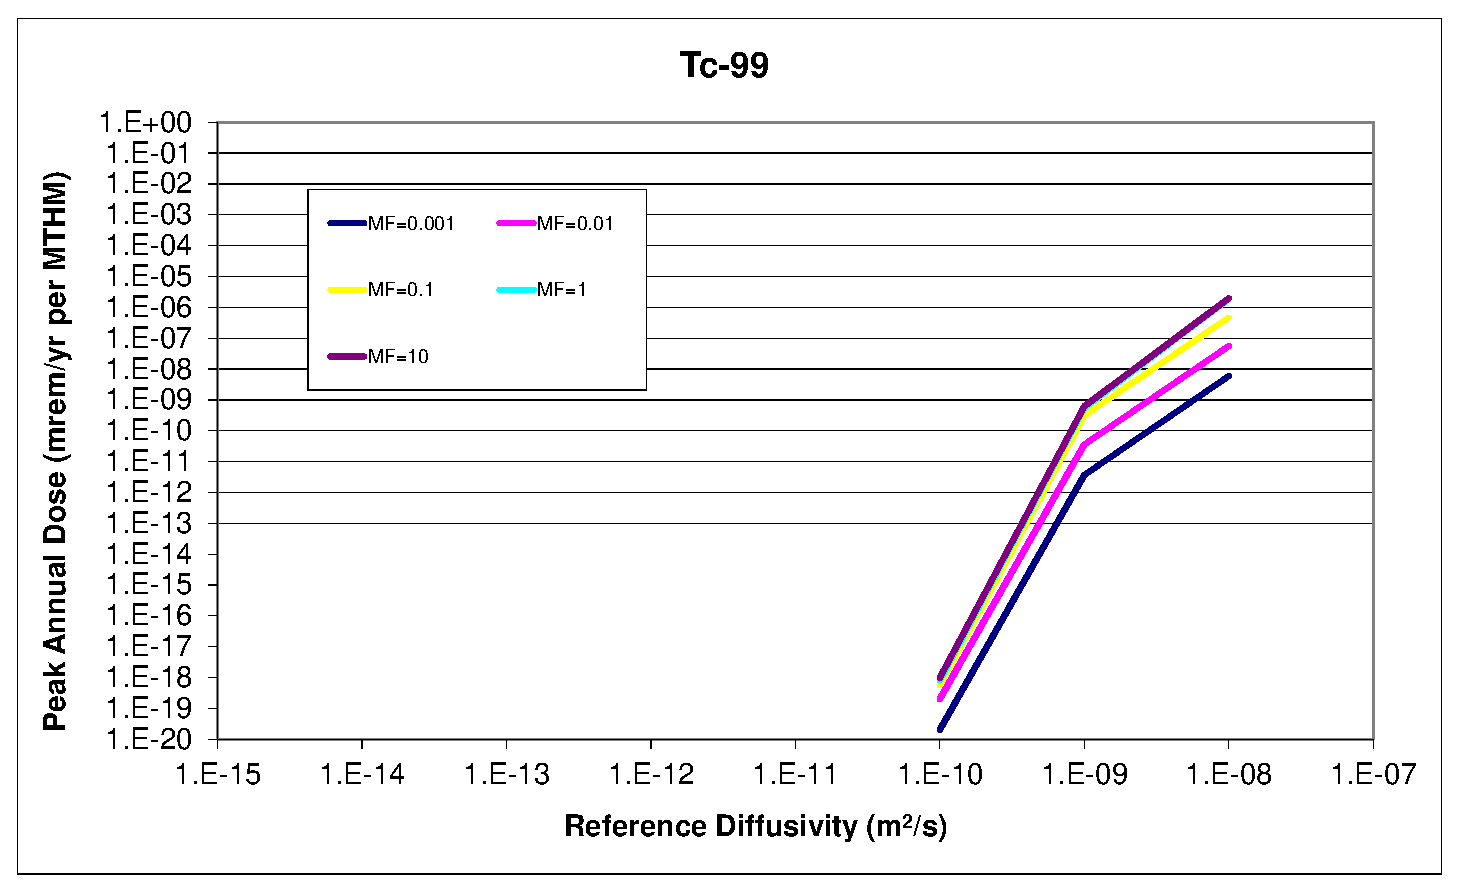
\includegraphics[width=\linewidth]{./chapters/nuclide_sensitivity/clay/DiffCoeffAndInvEBSFail/Tc-99.eps}
\caption{$^{99}Tc$ relative diffusivity sensitivity.} 
\label{fig:DCInvTc99}
\end{figure}

\begin{figure}[ht!]
\centering
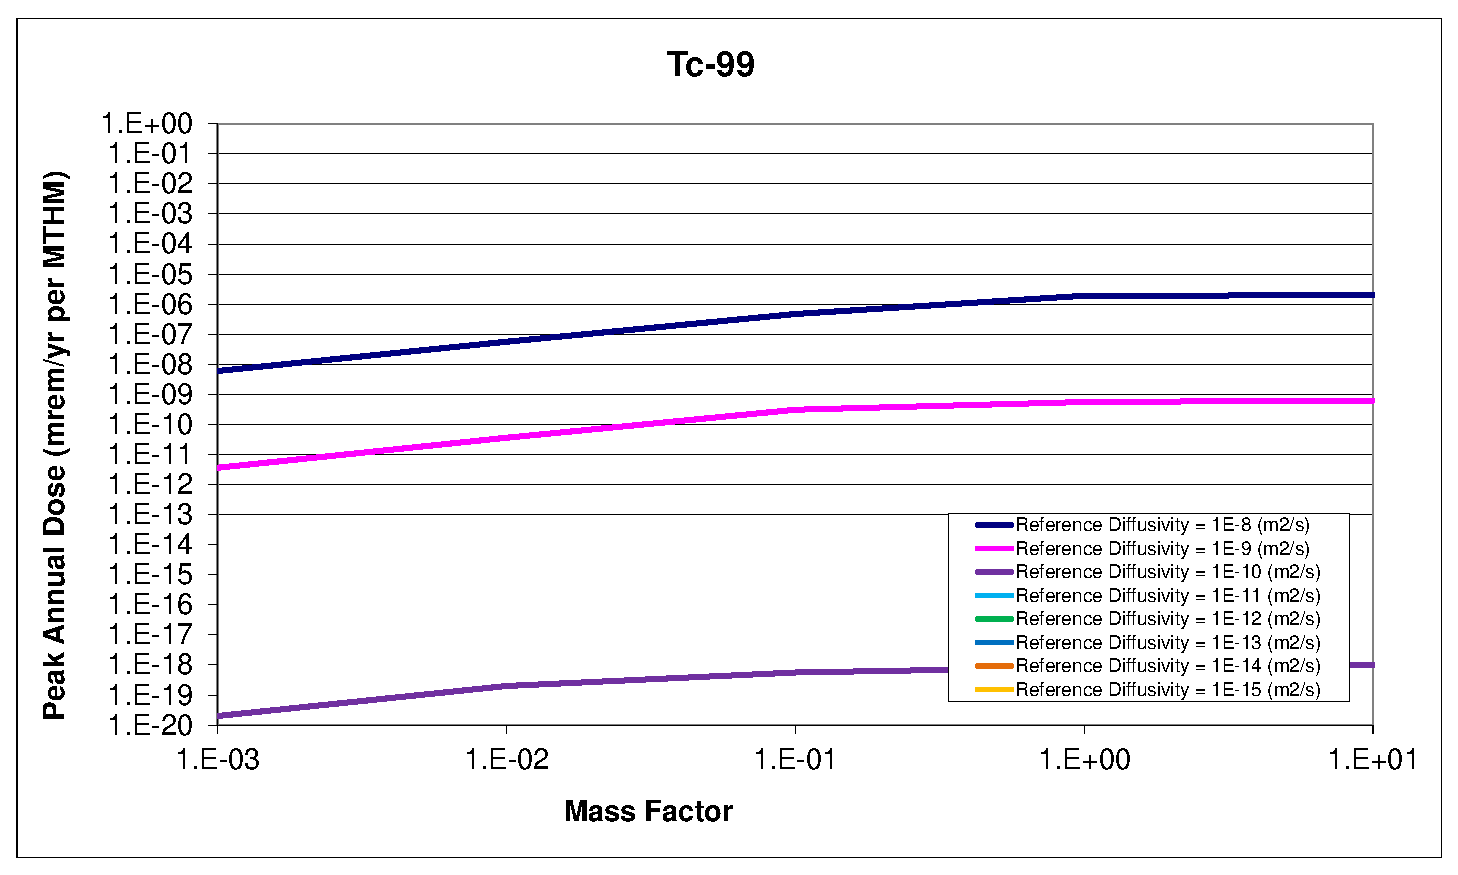
\includegraphics[width=\linewidth]{./chapters/nuclide_sensitivity/clay/DiffCoeffAndInvEBSFail/Tc-99-MF.eps}
\caption{$^{99}Tc$ mass factor sensitivity.}
\label{fig:DCInvTc99MF}
\end{figure}


\begin{figure}[ht!]
\centering
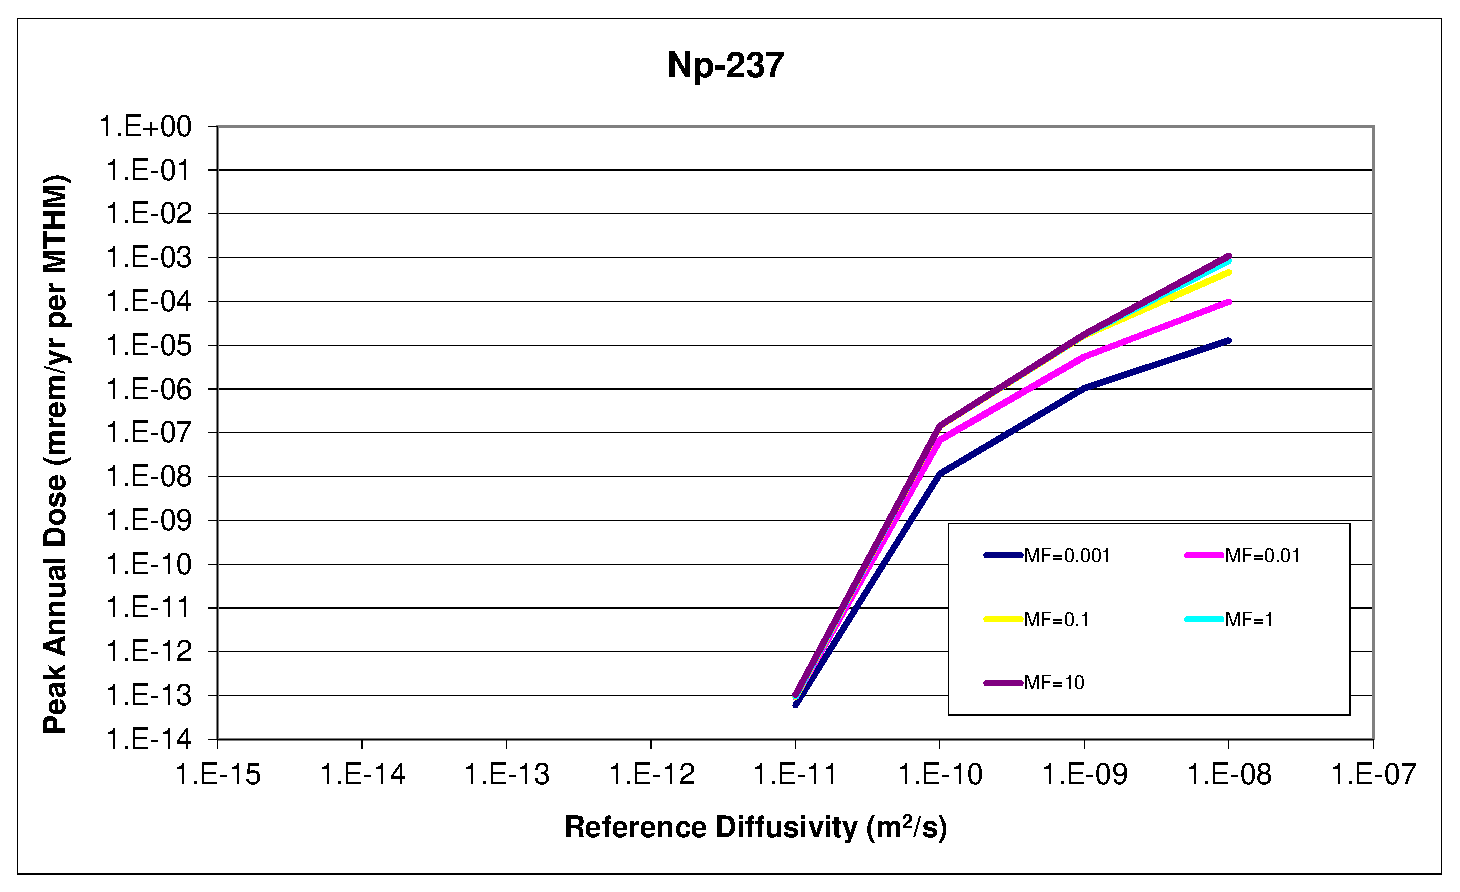
\includegraphics[width=\linewidth]{./chapters/nuclide_sensitivity/clay/DiffCoeffAndInvEBSFail/Np-237.eps}
\caption{$^{237}Np$ relative diffusivity sensitivity.} 
\label{fig:DCInvNp237}
\end{figure}

\begin{figure}[ht!]
\centering
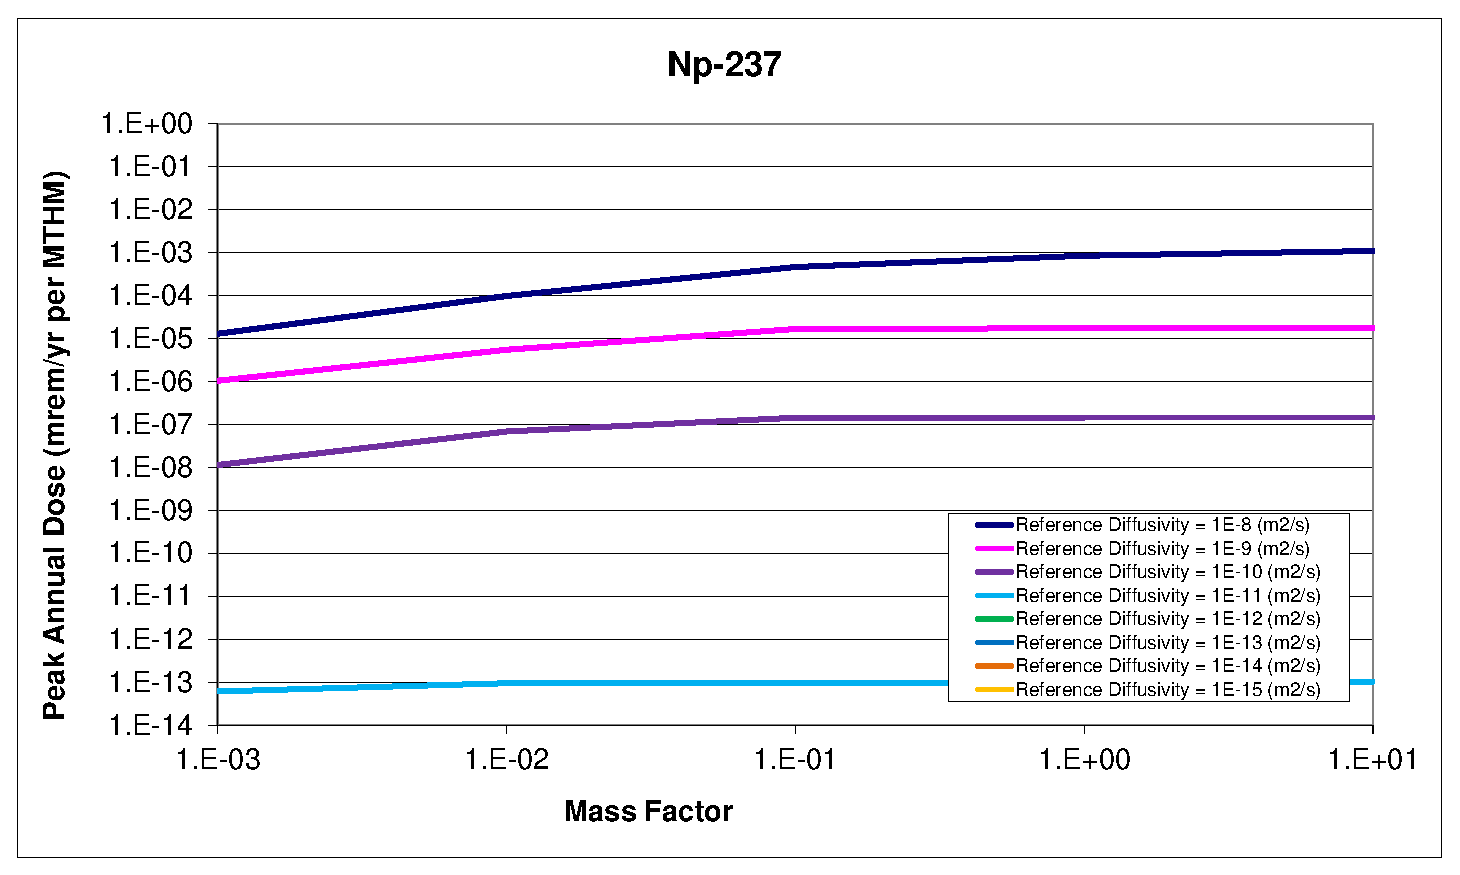
\includegraphics[width=\linewidth]{./chapters/nuclide_sensitivity/clay/DiffCoeffAndInvEBSFail/Np-237-MF.eps}
\caption{$^{237}Np$ mass factor sensitivity.}
\label{fig:DCInvNp237MF}
\end{figure}



\clearpage







\section{Spacing Thermal Transport Sensitivity Studies}\label{sec:spacing}


